%
\documentclass{beamer}
\usepackage{amssymb,amsmath,amsfonts,graphicx}
\usepackage[english]{babel}
\usepackage{graphics}
\usepackage{beamerthemesplit}
\usepackage{beamerthemeshadow}
\usepackage[latin1]{inputenc}
\usefonttheme{professionalfonts}
\usepackage{times}
\usepackage{amsmath}
\usecolortheme{whale}
\usepackage{enumerate}
\usepackage{amssymb}
\setcounter{tocdepth}{3}
\usepackage{graphicx}
\usepackage{epstopdf}
\usepackage{times}
\usepackage{subfigure}
\usepackage{color}
\usepackage{amsbsy}
\usepackage{amsmath}
\usepackage{amsfonts}
\usepackage{amssymb}
\usepackage{epsfig}
\usepackage{tabulary}
\usepackage{wrapfig}
\usepackage[noadjust]{cite}
%
%%%%%%%%%%%%%%%%%%%%%%%%%%%%%%%%%%%%%%%%%%%%%%%%%%%%%%%%%%%%%%%%%%
% General
%%%%%%%%%%%%%%%%%%%%%%%%%%%%%%%%%%%%%%%%%%%%%%%%%%%%%%%%%%%%%%%%%%
\newfont{\msym}{msbm10}
\newcommand{\reals}{\mathbb{R}}%Re}%{mbox{\msym R}}
\newcommand{\half}{\frac{1}{2}}       
\newcommand{\sign}{{\rm sign}}
\newcommand{\paren}[1]{\left({#1}\right)}
\newcommand{\brackets}[1]{\left[{#1}\right]}
\newcommand{\braces}[1]{\left\{{#1}\right\}}
\newcommand{\ceiling}[1]{\left\lceil{#1}\right\rceil}
\newcommand{\abs}[1]{\left\vert{#1}\right\vert}
\newcommand{\tr}{{\rm Tr}}
\newcommand{\pr}[1]{{\rm Pr}\left[{#1}\right]}
\newcommand{\prp}[2]{{\rm Pr}_{#1}\left[{#2}\right]}
\newcommand{\Exp}[1]{{\rm E}\left[{#1}\right]}
\newcommand{\Expp}[2]{{\rm E}_{#1}\left[{#2}\right]}
\newcommand{\eqdef}{\stackrel{\rm def}{=}}
\newcommand{\comdots}{, \ldots ,}
\newcommand{\true}{\texttt{True}}
\newcommand{\false}{\texttt{False}}
\newcommand{\mcal}[1]{{\mathcal{#1}}}
\newcommand{\argmin}[1]{\underset{#1}{\mathrm{argmin}} \:}
\newcommand{\normt}[1]{\left\Vert {#1} \right\Vert^2}
\newcommand{\step}[1]{\left[#1\right]_+}
\newcommand{\1}[1]{[\![{#1}]\!]}
\newcommand{\diag}{{\textrm{diag}}}
%\newcommand{\det}{{\textrm{det}}}
\newcommand{\KL}{{\textrm{D}_{\textrm{KL}}}}
\newcommand{\IS}{{\textrm{D}_{\textrm{IS}}}}
\newcommand{\EU}{{\textrm{D}_{\textrm{EU}}}}
\newcommand{\lloss}{\ell} % label loss
\newcommand{\closs}{\hat\ell} % classifier loss
\newcommand{\st}{\textrm{s.t.}} % such that / subject to

%%%%%%%%%%%%%%%%%%%%%%%%%%%%%%%%%%%%%%%%%%%%%%%%%%%%%%%%%%
% Control symbols
%%%%%%%%%%%%%%%%%%%%%%%%%%%%%%%%%%%%%%%%%%%%%%%%%%%%%%%%%%
\newcommand{\leftmarginpar}[1]{\marginpar[#1]{}}
\newcommand{\figline}{\rule{0.50\textwidth}{0.5pt}}
\newcommand{\pseudocodefont}{\normalsize}
\newcommand{\nolineskips}{
\setlength{\parskip}{0pt}
\setlength{\parsep}{0pt}
\setlength{\topsep}{0pt}
\setlength{\partopsep}{0pt}
\setlength{\itemsep}{0pt}}

%%%%%%%%%%%%%%%%%%%%%%%%%%%%%%%%%%%%%%%%%%%%%%%%%%%%%%%%%%%
% Equations and references
%%%%%%%%%%%%%%%%%%%%%%%%%%%%%%%%%%%%%%%%%%%%%%%%%%%%%%%%%%%
\newcommand{\beq}[1]{\begin{equation}\label{#1}}
\newcommand{\eeq}{\end{equation}}
\newcommand{\beqa}{\begin{eqnarray}}
\newcommand{\eeqa}{\end{eqnarray}}
%\renewcommand{\eqref}[1]{Eq.~(\ref{#1})}
\newcommand{\exmref}[1]{Example~\ref{#1}} 
\newcommand{\sthmref}[1]{Thm.~\ref{#1}}  
\newcommand{\remref}[1]{Remark~\ref{#1}} 
\newcommand{\claimref}[1]{Claim~\ref{#1}} 
\newcommand{\corref}[1]{Corollary~\ref{#1}} 
\newcommand{\scorref}[1]{Cor.~\ref{#1}} 
\newcommand{\tran}[1]{{#1}^{\top}}
\newcommand{\norm}{\mcal{N}}
\newcommand{\eqsref}[1]{Eqns.~(\ref{#1})}

% Alex's macros

\newcommand{\chaplabel}[1]{\label{chap:#1}}
\newcommand{\chapref}[1]{Chapter~\ref{chap:#1}}

\newcommand{\seclabel}[1]{\label{sec:#1}}
\newcommand{\secref}[1]{Section~\ref{sec:#1}}

\newcommand{\applabel}[1]{\label{app:#1}}
\newcommand{\appref}[1]{Appendix~\ref{app:#1}} 

\newcommand{\figlabel}[1]{\label{fig:#1}}
\newcommand{\figref}[1]{Figure~\ref{fig:#1}}

\newcommand{\tablabel}[1]{\label{tab:#1}}
\newcommand{\tabref}[1]{Table~\ref{tab:#1}}

\newcommand{\eqlabel}[1]{\label{eq:#1}}
\renewcommand{\eqref}[1]{Equation~(\ref{eq:#1})}

\newcommand{\proplabel}[1]{\label{prop:#1}}
\newcommand{\propref}[1]{Proposition~\ref{prop:#1}}

\newcommand{\deflabel}[1]{\label{def:#1}}
\newcommand{\defref}[1]{Definition~\ref{def:#1}}

\newcommand{\lemlabel}[1]{\label{lem:#1}}
\newcommand{\lemref}[1]{Lemma~\ref{lem:#1}}

\newcommand{\thmlabel}[1]{\label{thm:#1}}
\newcommand{\thmref}[1]{Theorem~\ref{thm:#1}}

\newcommand{\alglabel}[1]{\label{alg:#1}}
\newcommand{\algref}[1]{Algorithm~\ref{alg:#1}}


%%%%%%%%%%%%%%%%%%%%%%%%%%%%%%%%%%%%%%%%%%%%%%%%%%%%%%%%%%%
% bold, up, down
%%%%%%%%%%%%%%%%%%%%%%%%%%%%%%%%%%%%%%%%%%%%%%%%%%%%%%%%%%%
\newcommand{\mb}[1]{{\boldsymbol{#1}}}
\newcommand{\up}[2]{{#1}^{#2}}
\newcommand{\dn}[2]{{#1}_{#2}}
\newcommand{\du}[3]{{#1}_{#2}^{#3}}
\renewcommand{\star}[1]{\up{#1}{*}}
\newcommand{\textl}[2]{{$\textrm{#1}_{\textrm{#2}}$}}


%%%%%%%%%%%%%%%%%%%%%%%%%%%%%%%%%%%%%%%%%%%%%%%%%%%%%%%%%%%
% vectors \va
%%%%%%%%%%%%%%%%%%%%%%%%%%%%%%%%%%%%%%%%%%%%%%%%%%%%%%%%%%%
\newcommand{\vx}{\mb{x}} 
\newcommand{\vxi}[1]{\vx_{#1}}
\newcommand{\vxii}{\vxi{i}}

\newcommand{\yi}[1]{y_{#1}}
\newcommand{\yii}{\yi{i}}
\newcommand{\hy}{\hat{y}}
\newcommand{\hyi}[1]{\hat{y}_{#1}}
\newcommand{\hyii}{\hyi{i}}

\newcommand{\vy}{\mb{y}} 
\newcommand{\vyi}[1]{\vy_{#1}}
\newcommand{\vyii}{\vyi{i}}

\newcommand{\vn}{\mb{\nu}} 
\newcommand{\vni}[1]{\vn_{#1}}
\newcommand{\vnii}{\vni{i}}

\newcommand{\vmu}{\mb{\mu}}
\newcommand{\vmus}{{\vmu^*}}
\newcommand{\vmuts}{{\vmus}^{\top}}
\newcommand{\vmui}[1]{\vmu_{#1}}
\newcommand{\vmuii}{\vmui{i}}

\newcommand{\vmut}{\vmu^{\top}}
\newcommand{\vmuti}[1]{\vmut_{#1}}
\newcommand{\vmutii}{\vmuti{i}}

\newcommand{\vsigma}{\mb \sigma}
\newcommand{\msigma}{\Sigma}
\newcommand{\msigmas}{{\msigma^*}}
\newcommand{\msigmai}[1]{\msigma_{#1}}
\newcommand{\msigmaii}{\msigmai{i}}

\newcommand{\mups}{\Upsilon}
\newcommand{\mupss}{{\mups^*}}
\newcommand{\mupsi}[1]{\mups_{#1}}
\newcommand{\mupsii}{\mupsi{i}}
\newcommand{\upssl}{\upsilon^*_l}


\newcommand{\vu}{\mb{u}} 
\newcommand{\vut}{\tran{\vu}}
\newcommand{\vui}[1]{\vu_{#1}}
\newcommand{\vuti}[1]{\vut_{#1}}
\newcommand{\hvu}{\hat{\vu}}
\newcommand{\hvut}{\tran{\hvu}}
\newcommand{\hvur}[1]{\hvu_{#1}}
\newcommand{\hvutr}[1]{\hvut_{#1}}
\newcommand{\vw}{\mb{w}} 
\newcommand{\vwi}[1]{\vw_{#1}}
\newcommand{\vwii}{\vwi{i}}

\newcommand{\vwt}{\tran{\vw}}
\newcommand{\vwti}[1]{\vwt_{#1}}
\newcommand{\vwtii}{\vwti{i}}

\newcommand{\vv}{\mb{v}} 
\newcommand{\vvt}{\tran{\vv}}

\newcommand{\vvi}[1]{\vv_{#1}}
\newcommand{\vvti}[1]{\vvt_{#1}}
\newcommand{\lambdai}[1]{\lambda_{#1}}
\newcommand{\Lambdai}[1]{\Lambda_{#1}}

\newcommand{\vxt}{\tran{\vx}}
\newcommand{\hvx}{\hat{\vx}}
\newcommand{\hvxi}[1]{\hvx_{#1}}
\newcommand{\hvxii}{\hvxi{i}}
\newcommand{\hvxt}{\tran{\hvx}}
\newcommand{\hvxti}[1]{\hvxt_{#1}}
\newcommand{\hvxtii}{\hvxti{i}}
\newcommand{\vxti}[1]{\vxt_{#1}}
\newcommand{\vxtii}{\vxti{i}}

%%%%%%%%%%%%%%%%%%%%%%%%%%%%%%%%%%%%%%%%%%%%%%%%%%%%%%%%%%%%%%%%%
% Matrices (\mA)
%%%%%%%%%%%%%%%%%%%%%%%%%%%%%%%%%%%%%%%%%%%%%%%%%%%%%%%%%%%%%%%%%


\renewcommand{\mp}{P}
\newcommand{\mpd}{\mp^{(d)}}
\newcommand{\mpt}{\mp^T}
\newcommand{\tmp}{\tilde{\mp}}
\newcommand{\mpi}[1]{\mp_{#1}}
\newcommand{\mpti}[1]{\mpt_{#1}}
\newcommand{\mptii}{\mpti{i}}
\newcommand{\mpii}{\mpi{i}}
\newcommand{\mps}{Q}
\newcommand{\mpsi}[1]{\mps_{#1}}
\newcommand{\mpsii}{\mpsi{i}}
\newcommand{\tmpt}{\tmp^T}
\newcommand{\mz}{Z}
\newcommand{\mv}{V}
\newcommand{\mvi}[1]{\mv_{#1}}
\newcommand{\mvt}{V^T}
\newcommand{\mvti}[1]{\mvt_{#1}}
\newcommand{\mzt}{\mz^T}
\newcommand{\tmz}{\tilde{\mz}}
\newcommand{\tmzt}{\tmz^T}
\newcommand{\mx}{\mathbf{X}}
\newcommand{\ma}{\mathbf{A}}
\newcommand{\mxs}[1]{\mx_{#1}}


\newcommand{\mxi}[1]{\textrm{diag}^2\paren{\vxi{#1}}}
\newcommand{\mxii}{\mxi{i}}

%\newcommand{\mxi}[1]{\mx_{#1}}
%\newcommand{\mxii}{\mxi{i}}
\newcommand{\hmx}{\hat{\mx}}
\newcommand{\hmxi}[1]{\hmx_{#1}}
\newcommand{\hmxii}{\hmxi{i}}
\newcommand{\hmxt}{\hmx^T}
\newcommand{\mxt}{\mx^\top}
\newcommand{\mi}{I}
\newcommand{\mq}{Q}
\newcommand{\mqt}{\mq^T}
\newcommand{\mlam}{\Lambda}
%\newcommand{\ma}{A}
%\newcommand{\ms}{S}
%\newcommand{\mt}{T}

%%%%%%%%%%%%%%%%%%%%%%%%%%%%%%%%%%%%%%%%%%%%%%%%%%%%%%%%%%%
% mathcal 
%%%%%%%%%%%%%%%%%%%%%%%%%%%%%%%%%%%%%%%%%%%%%%%%%%%%%%%%%%%
\renewcommand{\L}{\mcal{L}}
\newcommand{\R}{\mcal{R}}
\newcommand{\X}{\mcal{X}}
\newcommand{\Y}{\mcal{Y}}
\newcommand{\F}{\mcal{F}}
\newcommand{\nur}[1]{\nu_{#1}}
\newcommand{\lambdar}[1]{\lambda_{#1}}
\newcommand{\gammai}[1]{\gamma_{#1}}
\newcommand{\gammaii}{\gammai{i}}
\newcommand{\alphai}[1]{\alpha_{#1}}
\newcommand{\alphaii}{\alphai{i}}
\newcommand{\lossp}[1]{\ell_{#1}}
\newcommand{\eps}{\epsilon}
\newcommand{\epss}{\eps^*}
\newcommand{\lsep}{\lossp{\eps}}
\newcommand{\lseps}{\lossp{\epss}}
\newcommand{\T}{\mcal{T}}

%%%%%%%%%%%%%%%%%%%%%%%%%%%%%%%%%%%%%%%%%%%%%%%%%%%%%%%%%%%
% Notes
%%%%%%%%%%%%%%%%%%%%%%%%%%%%%%%%%%%%%%%%%%%%%%%%%%%%%%%%%%%
\newcommand{\kc}[1]{\begin{center}\fbox{\parbox{3in}{{\textcolor{green}{KC: #1}}}}\end{center}}
\newcommand{\fp}[1]{\begin{center}\fbox{\parbox{3in}{{\textcolor{red}{FP: #1}}}}\end{center}}
\newcommand{\md}[1]{\begin{center}\fbox{\parbox{3in}{{\textcolor{blue}{MD: #1}}}}\end{center}}
\newcommand{\ak}[1]{\begin{center}\fbox{\parbox{3in}{{\textcolor{yellow}{AK: #1}}}}\end{center}}




\newcommand{\newstuffa}[2]{#2}
\newcommand{\newstufffroma}[1]{}
\newcommand{\newstufftoa}{}
%\newcommand{\newstuffa}[2]{~\\{\color{MyRed} #1:\\ }{\textcolor{MyGray}{#2}~\\}}
%\newcommand{\newstufffroma}[1]{~\\{\color{MyRed} #1:\\ }\color{MyGray}}
%\newcommand{\newstufftoa}{\color{black}}

\newcommand{\newstuff}[2]{#2}
\newcommand{\newstufffrom}[1]{}
\newcommand{\newstuffto}{}
\newcommand{\oldnote}[2]{}

%%%%\newcommand{\comment}[1]{}
\newcommand{\commentout}[1]{}
\newcommand{\mypar}[1]{\medskip\noindent{\bf #1}}


%%%%%%%%%%%%%%%%%%%%%%%%%%%%%%%%%%%%%%%%%%%%%%%%%%%%%%%%%%%
% other
%%%%%%%%%%%%%%%%%%%%%%%%%%%%%%%%%%%%%%%%%%%%%%%%%%%%%%%%%%%
% inner products
\newcommand{\inner}[2]{\left< {#1} , {#2} \right>}
\newcommand{\kernel}[2]{K\left({#1},{#2} \right)}
\newcommand{\tprr}{\tilde{p}_{rr}}
\newcommand{\hxr}{\hat{x}_{r}}
\newcommand{\projalg}{{PST }}%{\tt Projection }}
\newcommand{\projealg}[1]{$\textrm{PST}_{#1}~$}%{\tt Projection }}
\newcommand{\gradalg}{{GST }}%\tt Gradient }}



\newcounter {mySubCounter}
\newcommand {\twocoleqn}[4]{
  \setcounter {mySubCounter}{0} %
  \let\OldTheEquation \theequation %
  \renewcommand {\theequation }{\OldTheEquation \alph {mySubCounter}}%
  \noindent \hfill%
  \begin{minipage}{.40\textwidth}
\vspace{-0.6cm}
    \begin{equation}\refstepcounter{mySubCounter}
      #1 
    \end {equation}
  \end {minipage}
~~~~~~
%\hfill %
  \addtocounter {equation}{ -1}%
  \begin{minipage}{.40\textwidth}
\vspace{-0.6cm}
    \begin{equation}\refstepcounter{mySubCounter}
      #3 
    \end{equation}
  \end{minipage}%
  \let\theequation\OldTheEquation
}


\newcommand{\vzero}{\mb{0}} 

\newcommand{\smargin}{\mcal{M}}

\newcommand{\ai}[1]{A_{#1}}
\newcommand{\bi}[1]{B_{#1}}
\newcommand{\aii}{\ai{i}}
\newcommand{\bii}{\bi{i}}
\newcommand{\betai}[1]{\beta_{#1}}
\newcommand{\betaii}{\betai{i}}
\newcommand{\mar}{M}
\newcommand{\mari}[1]{\mar_{#1}}
\newcommand{\marii}{\mari{i}}
\newcommand{\nmari}[1]{m_{#1}}
\newcommand{\nmarii}{\nmari{i}}


%\newcommand{\erf}{\mathrm{erf}}
\newcommand{\erf}{\Phi}


\newcommand{\var}{V}
\newcommand{\vari}[1]{\var_{#1}}
\newcommand{\varii}{\vari{i}}

\newcommand{\varb}{v}
\newcommand{\varbi}[1]{\varb_{#1}}
\newcommand{\varbii}{\varbi{i}}

%\newcommand{\vara}{v^+}
\newcommand{\vara}{u}
\newcommand{\varai}[1]{\vara_{#1}}
\newcommand{\varaii}{\varai{i}}

\newcommand{\marb}{m}
\newcommand{\marbi}[1]{\marb_{#1}}
\newcommand{\marbii}{\marbi{i}}

\newcommand{\algname}{{AROW}}
\newcommand{\rlsname}{{RLS}}
\newcommand{\mrlsname}{{MRLS}}


%\newcommand{phi1}{{1+\frac{\phi}{2}}}
\newcommand{\phia}{\psi}
\newcommand{\phib}{\xi}


\newcommand{\amsigmaii}{\tilde{\msigma}_i}
\newcommand{\amsigmai}[1]{\tilde{\msigma}_{#1}}
\newcommand{\avmuii}{\tilde{\vmu}_i}
\newcommand{\avmui}[1]{\tilde{\vmu}_{#1}}
\newcommand{\amarbii}{\tilde{\marb}_i}
\newcommand{\avarbii}{\tilde{\varb}_i}
\newcommand{\avaraii}{\tilde{\vara}_i} 
\newcommand{\aalphaii}{\tilde{\alpha}_i}

\newcommand{\svar}{v}
\newcommand{\smar}{m}
\newcommand{\nsmar}{\bar{m}}

\newcommand{\vnu}{\mb{\nu}}
\newcommand{\vnut}{\vnu^\top}
\newcommand{\vz}{\mb{z}} 
\newcommand{\vZ}{\mb{Z}}
\newcommand{\fphi}{f_{\phi}}
\newcommand{\gphi}{g_{\phi}}

%%% Local Variables: 
%%% mode: latex
%%% TeX-master: "nips2007"
%%% End: 


\newcommand{\vtmui}[1]{\tilde{\vmu}_{#1}}
\newcommand{\vtmuii}{\vtmui{i}}


\newcommand{\zetai}[1]{\zeta_{#1}}
\newcommand{\zetaii}{\zetai{i}}



%%%%%%

\newcommand{\vstate}{\bf{s}}
\newcommand{\vstatet}[1]{\vstate_{#1}}
\newcommand{\vstatett}{\vstatet{t}}

\newcommand{\mtran}{\bf{\Phi}}
\newcommand{\mtrant}[1]{\mtran_{#1}}
\newcommand{\mtrantt}{\mtrant{t}}

\newcommand{\vstatenoise}{\bf{\eta}}
\newcommand{\vstatenoiset}[1]{\vstatenoise_{#1}}
\newcommand{\vstatenoisett}{\vstatenoiset{t}}


\newcommand{\vobser}{\bf{o}}
\newcommand{\vobsert}[1]{\vobser_{#1}}
\newcommand{\vobsertt}{\vobsert{t}}

\newcommand{\mobser}{\bf{H}}
\newcommand{\mobsert}[1]{\mobser_{#1}}
\newcommand{\mobsertt}{\mobsert{t}}

\newcommand{\vobsernoise}{\bf{\nu}}
\newcommand{\vobsernoiset}[1]{\vobsernoise_{#1}}
\newcommand{\vobsernoisett}{\vobsernoiset{t}}

\newcommand{\mstatenoisecov}{\bf{Q}}
\newcommand{\mstatenoisecovt}[1]{\mstatenoisecov_{#1}}
\newcommand{\mstatenoisecovtt}{\mstatenoisecovt{t}}

\newcommand{\mobsernoisecov}{\bf{R}}
\newcommand{\mobsernoisecovt}[1]{\mobsernoisecov_{#1}}
\newcommand{\mobsernoisecovtt}{\mobsernoisecovt{t}}



\newcommand{\vestate}{\bf{\hat{s}}}
\newcommand{\vestatet}[1]{\vestate_{#1}}
\newcommand{\vestatett}{\vestatet{t}}
\newcommand{\vestatept}[1]{\vestatet{#1}^+}
\newcommand{\vestatent}[1]{\vestatet{#1}^-}


\newcommand{\mcovar}{\bf{P}}
\newcommand{\mcovart}[1]{\mcovar_{#1}}
\newcommand{\mcovarpt}[1]{\mcovart{#1}^+}
\newcommand{\mcovarnt}[1]{\mcovart{#1}^-}

\newcommand{\mkalmangain}{\bf{K}}
\newcommand{\mkalmangaint}[1]{\mkalmangain_{#1}}


\newcommand{\vkalmangain}{\bf{\kappa}}
\newcommand{\vkalmangaint}[1]{\vkalmangain_{#1}}



\newcommand{\obsernoise}{{\nu}}
\newcommand{\obsernoiset}[1]{\obsernoise_{#1}}
\newcommand{\obsernoisett}{\obsernoiset{t}}

\newcommand{\obsernoisecov}{r}
\newcommand{\obsernoisecovt}[1]{\obsernoisecov_{#1}}
\newcommand{\obsernoisecovtt}{\obsernoisecov}%t{t}}


\newcommand{\obsnscv}{s}
\newcommand{\obsnscvt}[1]{\obsnscv_{#1}}
\newcommand{\obsnscvtt}{\obsnscvt{t}}


\newcommand{\Psit}[1]{\Psi_{#1}}
\newcommand{\Psitt}{\Psit{t}}

\newcommand{\Omegat}[1]{\Omega_{#1}}
\newcommand{\Omegatt}{\Omegat{t}}


\newcommand{\ellt}[1]{\ell_{#1}}
\newcommand{\gllt}[1]{g_{#1}}

\newcommand{\chit}[1]{\chi_{#1}}

\newcommand{\ms}{\mathcal{M}}
\newcommand{\us}{\mathcal{U}}
\newcommand{\as}{\mathcal{A}}

\newcommand{\mn}{M}
\newcommand{\un}{U}

\newcommand{\set}{S}
\newcommand{\seti}[1]{S_{#1}}

\newcommand{\obj}{\mcal{C}}

%
%  Macros for Thesis
%%%%%%%%%%%%%%%%%%%%%%%%%%%%%%%%%%%%%%%%%%%%%%%%%%%%%%%%%%%%%%%%%%%%%%%%%%%%%

 \newtheorem{theorem}{Theorem}
 \newtheorem{lemma}[theorem]{Lemma}
 \newtheorem{definition}[theorem]{Definition}
% \newtheorem{claim}[theorem]{Claim}
 \newtheorem{corollary}[theorem]{Corollary}


%\newtheorem{theorem}{Theorem}
%\newtheorem{lemma}[theorem]{Lemma}
%\newtheorem{corollary}[theorem]{Corollary}
%\newtheorem{definition}{Definition}
\newtheorem{Remark}{Remark}
%\newtheorem{claim}{Claim}
%\def\blackslug{\hbox{\hskip 1pt \vrule width 4pt height 8pt depth 1.5pt
%\hskip 1pt}}
\def\proof{\par\penalty-1000\vskip .5 pt\noindent{\bf Proof\/: }}
%\def\myproof{\par\penalty-1000\vskip .5 pt\noindent{\bf Proof~}}
\def\proofsketch{\par\penalty-1000\vskip .5 pt\noindent{\bf Proof sketch\/: }}
%\newcommand{\QED}{\hfill$\;\;\;\rule[0.1mm]{2mm}{2mm}$}
%\def\Proof{\par\penalty-1000\vskip .5 pt\noindent{\bf Proof\/: }}
\def\ProofSketch{\par\penalty-1000\vskip .1 pt\noindent{\bf Proof sketch\/: }}
\newcommand{\QED}{\hfill$\;\;\;\rule[0.1mm]{2mm}{2mm}$\\}
%\newenvironment{Proof}{{\bf Proof:}}{\noindent\bbox\vspace{0.1in}}

\newcommand{\todo}[1]{{~\\\bf TODO: {#1}}~\\}

%%%%%%%%%%%%%%%%%%%%%%%%%%%%%%%%%%%%%%%%%%%%%%%%%%%%%%%%%%%%%%%%%%
% General
%%%%%%%%%%%%%%%%%%%%%%%%%%%%%%%%%%%%%%%%%%%%%%%%%%%%%%%%%%%%%%%%%%
\newfont{\msym}{msbm10}
\newcommand{\reals}{\mathbb{R}}%Re}%{mbox{\msym R}}
\newcommand{\half}{\frac{1}{2}}
\newcommand{\sign}{{\rm sign}}
\newcommand{\paren}[1]{\left({#1}\right)}
\newcommand{\brackets}[1]{\left[{#1}\right]}
\newcommand{\braces}[1]{\left\{{#1}\right\}}
\newcommand{\ceiling}[1]{\left\lceil{#1}\right\rceil}
\newcommand{\abs}[1]{\left\vert{#1}\right\vert}
\newcommand{\tr}{{\rm Tr}}
\newcommand{\pr}[1]{{\rm Pr}\left[{#1}\right]}
\newcommand{\prp}[2]{{\rm Pr}_{#1}\left[{#2}\right]}
\newcommand{\Exp}[1]{{\rm E}\left[{#1}\right]}
\newcommand{\Expp}[2]{{\rm E}_{#1}\left[{#2}\right]}
\newcommand{\eqdef}{\stackrel{\rm def}{=}}
\newcommand{\comdots}{, \ldots ,}
\newcommand{\true}{\texttt{True}}
\newcommand{\false}{\texttt{False}}
\newcommand{\mcal}[1]{{\mathcal{#1}}}
\newcommand{\argmin}[1]{\underset{#1}{\mathrm{argmin}} \:}
\newcommand{\normt}[1]{\left\Vert {#1} \right\Vert^2}
\newcommand{\step}[1]{\left[#1\right]_+}
\newcommand{\1}[1]{[\![{#1}]\!]}
\newcommand{\diag}{{\textrm{diag}}}
%\newcommand{\det}{{\textrm{det}}}
\newcommand{\KL}{{\textrm{D}_{\textrm{KL}}}}
\newcommand{\IS}{{\textrm{D}_{\textrm{IS}}}}
\newcommand{\EU}{{\textrm{D}_{\textrm{EU}}}}

%%%%%%%%%%%%%%%%%%%%%%%%%%%%%%%%%%%%%%%%%%%%%%%%%%%%%%%%%%
% Control symbols
%%%%%%%%%%%%%%%%%%%%%%%%%%%%%%%%%%%%%%%%%%%%%%%%%%%%%%%%%%
\newcommand{\leftmarginpar}[1]{\marginpar[#1]{}}
\newcommand{\figline}{\rule{0.50\textwidth}{0.5pt}}
\newcommand{\pseudocodefont}{\normalsize}
\newcommand{\nolineskips}{
\setlength{\parskip}{0pt}
\setlength{\parsep}{0pt}
\setlength{\topsep}{0pt}
\setlength{\partopsep}{0pt}
\setlength{\itemsep}{0pt}}

%%%%%%%%%%%%%%%%%%%%%%%%%%%%%%%%%%%%%%%%%%%%%%%%%%%%%%%%%%%
% Equations and references
%%%%%%%%%%%%%%%%%%%%%%%%%%%%%%%%%%%%%%%%%%%%%%%%%%%%%%%%%%%
\newcommand{\beq}[1]{\begin{equation}\label{#1}}
\newcommand{\eeq}{\end{equation}}
\newcommand{\beqa}{\begin{eqnarray}}
\newcommand{\eeqa}{\end{eqnarray}}
\renewcommand{\eqref}[1]{Eq.~(\ref{#1})}
\newcommand{\secref}[1]{Sec.~\ref{#1}}
\newcommand{\figref}[1]{Fig.~\ref{#1}}
\newcommand{\exmref}[1]{Example~\ref{#1}}
\newcommand{\thmref}[1]{Theorem~\ref{#1}}
\newcommand{\sthmref}[1]{Thm.~\ref{#1}}
\newcommand{\defref}[1]{Definition~\ref{#1}}
\newcommand{\remref}[1]{Remark~\ref{#1}}
\newcommand{\chapref}[1]{Chapter~\ref{#1}}
\newcommand{\appref}[1]{Appendix~\ref{#1}}
\newcommand{\lemref}[1]{Lemma~\ref{#1}}
\newcommand{\propref}[1]{Proposition~\ref{#1}}
\newcommand{\claimref}[1]{Claim~\ref{#1}}
\newcommand{\corref}[1]{Corollary~\ref{#1}}
\newcommand{\scorref}[1]{Cor.~\ref{#1}}
\newcommand{\tabref}[1]{Table~\ref{#1}}
\newcommand{\tran}[1]{{#1}^{\top}}
\newcommand{\norm}{\mcal{N}}
\newcommand{\eqsref}[1]{Eqns.~(\ref{#1})}
\newcommand{\algoref}[1]{Alg.~\ref{#1}}

%%%%%%%%%%%%%%%%%%%%%%%%%%%%%%%%%%%%%%%%%%%%%%%%%%%%%%%%%%%
% bold, up, down
%%%%%%%%%%%%%%%%%%%%%%%%%%%%%%%%%%%%%%%%%%%%%%%%%%%%%%%%%%%
\newcommand{\mb}[1]{{\boldsymbol{#1}}}
\newcommand{\up}[2]{{#1}^{#2}}
\newcommand{\dn}[2]{{#1}_{#2}}
\newcommand{\du}[3]{{#1}_{#2}^{#3}}
\renewcommand{\star}[1]{\up{#1}{*}}
\newcommand{\textl}[2]{{$\textrm{#1}_{\textrm{#2}}$}}


%%%%%%%%%%%%%%%%%%%%%%%%%%%%%%%%%%%%%%%%%%%%%%%%%%%%%%%%%%%
% vectors \va
%%%%%%%%%%%%%%%%%%%%%%%%%%%%%%%%%%%%%%%%%%%%%%%%%%%%%%%%%%%
\newcommand{\vx}{\mathbf{x}}
\newcommand{\vxi}[1]{\vx_{#1}}
\newcommand{\vxii}{\vxi{t}}

\newcommand{\ve}{\mathbf{e}}
\newcommand{\vei}[1]{\ve_{#1}}
\newcommand{\veii}{\vei{t}}
\newcommand{\vet}{\ve^{\top}}
\newcommand{\veti}[1]{\vet_{#1}}
\newcommand{\vetii}{\veti{i}}
\newcommand{\yi}[1]{y_{#1}}
\newcommand{\yii}{\yi{t}}
\newcommand{\hyi}[1]{\hat{y}_{#1}}
\newcommand{\hyii}{\hyi{i}}

\newcommand{\vy}{\mb{y}}
\newcommand{\vyi}[1]{\vy_{#1}}
\newcommand{\vyii}{\vyi{i}}

\newcommand{\vn}{\mb{\nu}}
\newcommand{\vni}[1]{\vn_{#1}}
\newcommand{\vnii}{\vni{i}}

\newcommand{\tvn}{\tilde{\mb{\nu}}}

\newcommand{\vmu}{\mb{\mu}}
\newcommand{\vmus}{{\vmu^*}}
\newcommand{\vmuts}{{\vmus}^{\top}}
\newcommand{\vmui}[1]{\vmu_{#1}}
\newcommand{\vmuii}{\vmui{i}}

\newcommand{\vmut}{\vmu^{\top}}
\newcommand{\vmuti}[1]{\vmut_{#1}}
\newcommand{\vmutii}{\vmuti{i}}

\newcommand{\vsigma}{\mb \sigma}
\newcommand{\msigma}{\mathbf{\Sigma}}
\newcommand{\msigmas}{{\msigma^*}}
\newcommand{\msigmai}[1]{\msigma_{#1}}
\newcommand{\msigmaii}{\msigmai{t}}

\newcommand{\mups}{\Upsilon}
\newcommand{\mupss}{{\mups^*}}
\newcommand{\mupsi}[1]{\mups_{#1}}
\newcommand{\mupsii}{\mupsi{i}}
\newcommand{\upssl}{\upsilon^*_l}


\newcommand{\vu}{\mathbf{u}}
\newcommand{\vut}{\tran{\vu}}
\newcommand{\vui}[1]{\vu_{#1}}
\newcommand{\vuti}[1]{\vut_{#1}}
\newcommand{\hvu}{\hat{\vu}}
\newcommand{\hvut}{\tran{\hvu}}
\newcommand{\hvur}[1]{\hvu_{#1}}
\newcommand{\hvutr}[1]{\hvut_{#1}}
\newcommand{\vw}{\mathbf{w}}
\newcommand{\vwi}[1]{\vw_{#1}}
\newcommand{\vwii}{\vwi{t}}
\newcommand{\vwti}[1]{\vwt_{#1}}
\newcommand{\vwt}{\tran{\vw}}

\newcommand{\tvw}{\tilde{\mathbf{w}}}
\newcommand{\tvwi}[1]{\tvw_{#1}}
\newcommand{\tvwii}{\tvwi{t}}

\newcommand{\vh}{\mb{h}}

\newcommand{\vv}{\mb{v}}
\newcommand{\vvt}{\tran{\vv}}

\newcommand{\vvi}[1]{\vv_{#1}}
\newcommand{\vvti}[1]{\vvt_{#1}}
\newcommand{\lambdai}[1]{\lambda_{#1}}
\newcommand{\Lambdai}[1]{\Lambda_{#1}}

\newcommand{\vxt}{\tran{\vx}}
\newcommand{\vxiit}{\vxi{i,t}}
\newcommand{\hvx}{\hat{\vx}}
\newcommand{\hvxi}[1]{\hvx_{#1}}
\newcommand{\hvxii}{\hvxi{i}}
\newcommand{\hvxt}{\tran{\hvx}}
\newcommand{\hvxti}[1]{\hvxt_{#1}}
\newcommand{\hvxtii}{\hvxti{i}}
\newcommand{\vxti}[1]{\vxt_{#1}}
\newcommand{\vxtii}{\vxti{i}}
\newcommand{\vwiit}{\vwi{i,t}}

\newcommand{\vb}{\mb{b}}
\newcommand{\vbt}{\tran{\vb}}
\newcommand{\vbi}[1]{\vb_{#1}}


\newcommand{\hvy}{\hat{\vy}}
\newcommand{\hvyi}[1]{\hvy_{#1}}
\newcommand{\yiit}{\yi{i,t}}

%%%%%%%%%%%%%%%%%%%%%%%%%%%%%%%%%%%%%%%%%%%%%%%%%%%%%%%%%%%%%%%%%
% Matrices (\mA)
%%%%%%%%%%%%%%%%%%%%%%%%%%%%%%%%%%%%%%%%%%%%%%%%%%%%%%%%%%%%%%%%%


\renewcommand{\mp}{P}
\newcommand{\mpd}{\mp^{(d)}}
\newcommand{\mpt}{\mp^T}
\newcommand{\tmp}{\tilde{\mp}}
\newcommand{\mpi}[1]{\mp_{#1}}
\newcommand{\mpti}[1]{\mpt_{#1}}
\newcommand{\mptii}{\mpti{i}}
\newcommand{\mpii}{\mpi{i}}
\newcommand{\mps}{Q}
\newcommand{\mpsi}[1]{\mps_{#1}}
\newcommand{\mpsii}{\mpsi{i}}
\newcommand{\tmpt}{\tmp^T}
\newcommand{\mz}{Z}
\newcommand{\mv}{V}
\newcommand{\mvi}[1]{\mv_{#1}}
\newcommand{\mvt}{V^T}
\newcommand{\mvti}[1]{\mvt_{#1}}
\newcommand{\mzt}{\mz^T}
\newcommand{\tmz}{\tilde{\mz}}
\newcommand{\tmzt}{\tmz^T}
\newcommand{\mx}{\mathbf{X}}
\newcommand{\ma}{\mathbf{A}}
\newcommand{\mxs}[1]{\mx_{#1}}


\newcommand{\mai}[1]{\ma_{#1}}
\newcommand{\mat}{\tran{\ma}}
\newcommand{\mati}[1]{\mat_{#1}}

\newcommand{\mc}{{C}}
\newcommand{\mci}[1]{\mc_{#1}}
\newcommand{\mcti}[1]{\mct_{#1}}


\newcommand{\md}{{\mathbf{D}}}
\newcommand{\mdi}[1]{\md_{#1}}
\newcommand{\mxi}[1]{\textrm{diag}^2\paren{\vxi{#1}}}
\newcommand{\mxii}{\mxi{i}}

%\newcommand{\mxi}[1]{\mx_{#1}}
%\newcommand{\mxii}{\mxi{i}}
\newcommand{\hmx}{\hat{\mx}}
\newcommand{\hmxi}[1]{\hmx_{#1}}
\newcommand{\hmxii}{\hmxi{i}}
\newcommand{\hmxt}{\hmx^T}
\newcommand{\mxt}{\mx^\top}
\newcommand{\mi}{\mathbf{I}}
\newcommand{\mq}{Q}
\newcommand{\mqt}{\mq^T}
\newcommand{\mlam}{\Lambda}
%\newcommand{\ma}{A}
%\newcommand{\ms}{S}
%\newcommand{\mt}{T}

%%%%%%%%%%%%%%%%%%%%%%%%%%%%%%%%%%%%%%%%%%%%%%%%%%%%%%%%%%%
% mathcal
%%%%%%%%%%%%%%%%%%%%%%%%%%%%%%%%%%%%%%%%%%%%%%%%%%%%%%%%%%%
\renewcommand{\L}{\mcal{L}}
%\newcommand{\R}{\mcal{R}}
\newcommand{\X}{\mcal{X}}
\newcommand{\Y}{\mcal{Y}}
\newcommand{\F}{\mcal{F}}
\newcommand{\nur}[1]{\nu_{#1}}
\newcommand{\lambdar}[1]{\lambda_{#1}}
\newcommand{\gammai}[1]{\gamma_{#1}}
\newcommand{\gammaii}{\gammai{i}}
\newcommand{\alphai}[1]{\alpha_{#1}}
\newcommand{\alphaii}{\alphai{i}}
\newcommand{\lossp}[1]{\ell_{#1}}
\newcommand{\eps}{\epsilon}
\newcommand{\epss}{\eps^*}
\newcommand{\lsep}{\lossp{\eps}}
\newcommand{\lseps}{\lossp{\epss}}
\newcommand{\T}{\mcal{T}}

%%%%%%%%%%%%%%%%%%%%%%%%%%%%%%%%%%%%%%%%%%%%%%%%%%%%%%%%%%%
% Notes
%%%%%%%%%%%%%%%%%%%%%%%%%%%%%%%%%%%%%%%%%%%%%%%%%%%%%%%%%%%
\newcommand{\kc}[1]{\begin{center}\fbox{\parbox{3in}{{\textcolor{green}{KC: #1}}}}\end{center}}
\newcommand{\edward}[1]{\begin{center}\fbox{\parbox{3in}{{\textcolor{red}{EM: #1}}}}\end{center}}
\newcommand{\nv}[1]{\begin{center}\fbox{\parbox{3in}{{\textcolor{blue}{NV: #1}}}}\end{center}}




\newcommand{\newstuffa}[2]{#2}
\newcommand{\newstufffroma}[1]{}
\newcommand{\newstufftoa}{}
%\newcommand{\newstuffa}[2]{~\\{\color{MyRed} #1:\\ }{\textcolor{MyGray}{#2}~\\}}
%\newcommand{\newstufffroma}[1]{~\\{\color{MyRed} #1:\\ }\color{MyGray}}
%\newcommand{\newstufftoa}{\color{black}}

\newcommand{\newstuff}[2]{#2}
\newcommand{\newstufffrom}[1]{}
\newcommand{\newstuffto}{}
\newcommand{\oldnote}[2]{}

%%%%\newcommand{\comment}[1]{}
\newcommand{\commentout}[1]{}
\newcommand{\mypar}[1]{\medskip\noindent{\bf #1}}


%%%%%%%%%%%%%%%%%%%%%%%%%%%%%%%%%%%%%%%%%%%%%%%%%%%%%%%%%%%
% other
%%%%%%%%%%%%%%%%%%%%%%%%%%%%%%%%%%%%%%%%%%%%%%%%%%%%%%%%%%%
% inner products
\newcommand{\inner}[2]{\left< {#1} , {#2} \right>}
\newcommand{\kernel}[2]{K\left({#1},{#2} \right)}
\newcommand{\tprr}{\tilde{p}_{rr}}
\newcommand{\hxr}{\hat{x}_{r}}
\newcommand{\projalg}{{PST }}%{\tt Projection }}
\newcommand{\projealg}[1]{$\textrm{PST}_{#1}~$}%{\tt Projection }}
\newcommand{\gradalg}{{GST }}%\tt Gradient }}



\newcounter {mySubCounter}
\newcommand {\twocoleqn}[4]{
  \setcounter {mySubCounter}{0} %
  \let\OldTheEquation \theequation %
  \renewcommand {\theequation }{\OldTheEquation \alph {mySubCounter}}%
  \noindent \hfill%
  \begin{minipage}{.40\textwidth}
\vspace{-0.6cm}
    \begin{equation}\refstepcounter{mySubCounter}
      #1
    \end {equation}
  \end {minipage}
~~~~~~
%\hfill %
  \addtocounter {equation}{ -1}%
  \begin{minipage}{.40\textwidth}
\vspace{-0.6cm}
    \begin{equation}\refstepcounter{mySubCounter}
      #3
    \end{equation}
  \end{minipage}%
  \let\theequation\OldTheEquation
}


\newcommand{\vzero}{\mb{0}}

\newcommand{\smargin}{\mcal{M}}

\newcommand{\ai}[1]{A_{#1}}
\newcommand{\bi}[1]{B_{#1}}
\newcommand{\aii}{\ai{i}}
\newcommand{\bii}{\bi{i}}
\newcommand{\betai}[1]{\beta_{#1}}
\newcommand{\betaii}{\betai{i}}
\newcommand{\mar}{M}
\newcommand{\mari}[1]{\mar_{#1}}
\newcommand{\marii}{\mari{i}}
\newcommand{\nmari}[1]{m_{#1}}
\newcommand{\nmarii}{\nmari{i}}


%\newcommand{\erf}{\mathrm{erf}}
\newcommand{\erf}{\Phi}


\newcommand{\var}{V}
\newcommand{\vari}[1]{\var_{#1}}
\newcommand{\varii}{\vari{i}}

\newcommand{\varb}{v}
\newcommand{\varbi}[1]{\varb_{#1}}
\newcommand{\varbii}{\varbi{i}}

%\newcommand{\vara}{v^+}
\newcommand{\vara}{u}
\newcommand{\varai}[1]{\vara_{#1}}
\newcommand{\varaii}{\varai{i}}

\newcommand{\marb}{m}
\newcommand{\marbi}[1]{\marb_{#1}}
\newcommand{\marbii}{\marbi{i}}

\newcommand{\algname}{{AROW}}
\newcommand{\rlsname}{{RLS}}
\newcommand{\mrlsname}{{MRLS}}


%\newcommand{phi1}{{1+\frac{\phi}{2}}}
\newcommand{\phia}{\psi}
\newcommand{\phib}{\xi}


\newcommand{\amsigmaii}{\tilde{\msigma}_t}
\newcommand{\amsigmai}[1]{\tilde{\msigma}_{#1}}
\newcommand{\avmuii}{\tilde{\vmu}_i}
\newcommand{\avmui}[1]{\tilde{\vmu}_{#1}}
\newcommand{\amarbii}{\tilde{\marb}_i}
\newcommand{\avarbii}{\tilde{\varb}_i}
\newcommand{\avaraii}{\tilde{\vara}_i}
\newcommand{\aalphaii}{\tilde{\alpha}_i}

\newcommand{\svar}{v}
\newcommand{\smar}{m}
\newcommand{\nsmar}{\bar{m}}

\newcommand{\vnu}{\mb{\nu}}
\newcommand{\vnut}{\vnu^\top}
\newcommand{\vz}{\mb{z}}
\newcommand{\vZ}{\mb{Z}}
\newcommand{\fphi}{f_{\phi}}
\newcommand{\gphi}{g_{\phi}}

%%% Local Variables:
%%% mode: latex
%%% TeX-master: "nips2007"
%%% End:


\newcommand{\vtmui}[1]{\tilde{\vmu}_{#1}}
\newcommand{\vtmuii}{\vtmui{i}}


\newcommand{\zetai}[1]{\zeta_{#1}}
\newcommand{\zetaii}{\zetai{i}}



%%%%%%

\newcommand{\vstate}{\bf{s}}
\newcommand{\vstatet}[1]{\vstate_{#1}}
\newcommand{\vstatett}{\vstatet{t}}

\newcommand{\mtran}{\bf{\Phi}}
\newcommand{\mtrant}[1]{\mtran_{#1}}
\newcommand{\mtrantt}{\mtrant{t}}

\newcommand{\vstatenoise}{\bf{\eta}}
\newcommand{\vstatenoiset}[1]{\vstatenoise_{#1}}
\newcommand{\vstatenoisett}{\vstatenoiset{t}}


\newcommand{\vobser}{\bf{o}}
\newcommand{\vobsert}[1]{\vobser_{#1}}
\newcommand{\vobsertt}{\vobsert{t}}

\newcommand{\mobser}{\bf{H}}
\newcommand{\mobsert}[1]{\mobser_{#1}}
\newcommand{\mobsertt}{\mobsert{t}}

\newcommand{\vobsernoise}{\bf{\nu}}
\newcommand{\vobsernoiset}[1]{\vobsernoise_{#1}}
\newcommand{\vobsernoisett}{\vobsernoiset{t}}

\newcommand{\mstatenoisecov}{\bf{Q}}
\newcommand{\mstatenoisecovt}[1]{\mstatenoisecov_{#1}}
\newcommand{\mstatenoisecovtt}{\mstatenoisecovt{t}}

\newcommand{\mobsernoisecov}{\bf{R}}
\newcommand{\mobsernoisecovt}[1]{\mobsernoisecov_{#1}}
\newcommand{\mobsernoisecovtt}{\mobsernoisecovt{t}}



\newcommand{\vestate}{\bf{\hat{s}}}
\newcommand{\vestatet}[1]{\vestate_{#1}}
\newcommand{\vestatett}{\vestatet{t}}
\newcommand{\vestatept}[1]{\vestatet{#1}^+}
\newcommand{\vestatent}[1]{\vestatet{#1}^-}


\newcommand{\mcovar}{\bf{P}}
\newcommand{\mcovart}[1]{\mcovar_{#1}}
\newcommand{\mcovarpt}[1]{\mcovart{#1}^+}
\newcommand{\mcovarnt}[1]{\mcovart{#1}^-}

\newcommand{\mkalmangain}{\bf{K}}
\newcommand{\mkalmangaint}[1]{\mkalmangain_{#1}}


\newcommand{\vkalmangain}{\bf{\kappa}}
\newcommand{\vkalmangaint}[1]{\vkalmangain_{#1}}



\newcommand{\obsernoise}{{\nu}}
\newcommand{\obsernoiset}[1]{\obsernoise_{#1}}
\newcommand{\obsernoisett}{\obsernoiset{t}}

\newcommand{\obsernoisecov}{r}
\newcommand{\obsernoisecovt}[1]{\obsernoisecov_{#1}}
\newcommand{\obsernoisecovtt}{\obsernoisecov}%t{t}}


\newcommand{\obsnscv}{s}
\newcommand{\obsnscvt}[1]{\obsnscv_{#1}}
\newcommand{\obsnscvtt}{\obsnscvt{t}}


\newcommand{\Psit}[1]{\Psi_{#1}}
\newcommand{\Psitt}{\Psit{t}}

\newcommand{\Omegat}[1]{\Omega_{#1}}
\newcommand{\Omegatt}{\Omegat{t}}


\newcommand{\ellt}[1]{\ell_{#1}}
\newcommand{\gllt}[1]{g_{#1}}

\newcommand{\chit}[1]{\chi_{#1}}

\newcommand{\ms}{\mathcal{M}}
\newcommand{\us}{\mathcal{U}}
\newcommand{\as}{\mathcal{A}}

\newcommand{\mn}{M}
\newcommand{\un}{U}

\newcommand{\set}{S}
\newcommand{\seti}[1]{S_{#1}}

\newcommand{\obj}{\mcal{C}}

\newcommand{\dta}[3]{d_{#3}\paren{#1,#2}}

\newcommand{\coa}{a}
\newcommand{\coc}{c}
\newcommand{\cob}{b}
\newcommand{\cor}{r}
\newcommand{\conu}{\nu}

\newcommand{\coat}[1]{\coa_{#1}}
\newcommand{\coct}[1]{\coc_{#1}}
\newcommand{\cobt}[1]{\cob_{#1}}
\newcommand{\cort}[1]{\cor_{#1}}
\newcommand{\conut}[1]{\conu_{#1}}


\newcommand{\coatt}{\coat{t}}
\newcommand{\coctt}{\coct{t}}
\newcommand{\cobtt}{\cobt{t}}
\newcommand{\cortt}{\cort{t}}
\newcommand{\conutt}{\conut{t}}

\newcommand{\rb}{R_B}
\newcommand{\proj}{\textrm{proj}}



\usetheme{Frankfurt}
%\usetheme{Warsaw}
%\setbeamertemplate{footline}[frame number]
  \useoutertheme{infolines}
    \usefonttheme[onlysmall]{structurebold}

\title []{Multi-task Learning with a  \\Shared Annotator}    % Enter
\author [H. Cohen and K. Crammer]{Haim Cohen \and \newline\newline  Supervised by Prof. Koby Crammer\newline\newline}

\institute [Technion]{Faculty of Electrical Engineering, Technion\\
Israel Institute of Technology}

\date[March 30th, 2016]{30.3.2016}

\usepackage[normalem]{ulem}

\begin{document}

\maketitle
\section{Introduction}

\begin{frame}{Outline}
  \tableofcontents[pausesections]
\end{frame}


\begin{frame}{Online Learning}
\begin{itemize}
\item Input  comes in sequence \newline
\item Feedback after prediction  \newline
\item   Uses when  : \newline
\begin{itemize}
\item Data comes in sequence \newline
\item Big data \newline
\end{itemize}
\item Examples: stock market, advertisement, content recommendation etc.\newline

\end{itemize}
\end{frame}


\begin{frame}{Online Learning}
\begin{itemize}
\item On each round:\newline
\begin{enumerate}
\item Instance $\vxi{t}$ is observed\newline
\item Prediction $\hat{y}_t$ is made\newline
\item Loss $\lossp{t}$ is suffered\newline
\item True value $y_t$ is revealed\newline
\item An update of the model is made\newline
\end{enumerate}
\item Loss types: zero-one, hinge, exponential, quadratic...
\end{itemize}
\end{frame}

\subsection{Problem statement}

\begin{frame}{Problem statement}
\begin{itemize}
\item $K$ binary learning tasks  in parallel\newline
\item Limited resources (limited bandwidth) \newline
\item Annotate one task at a time \newline

\item Examples: classify data news from many agencies\newline
\end{itemize}
\end{frame}


\begin{frame}{Problem statement - update}
\begin{center}
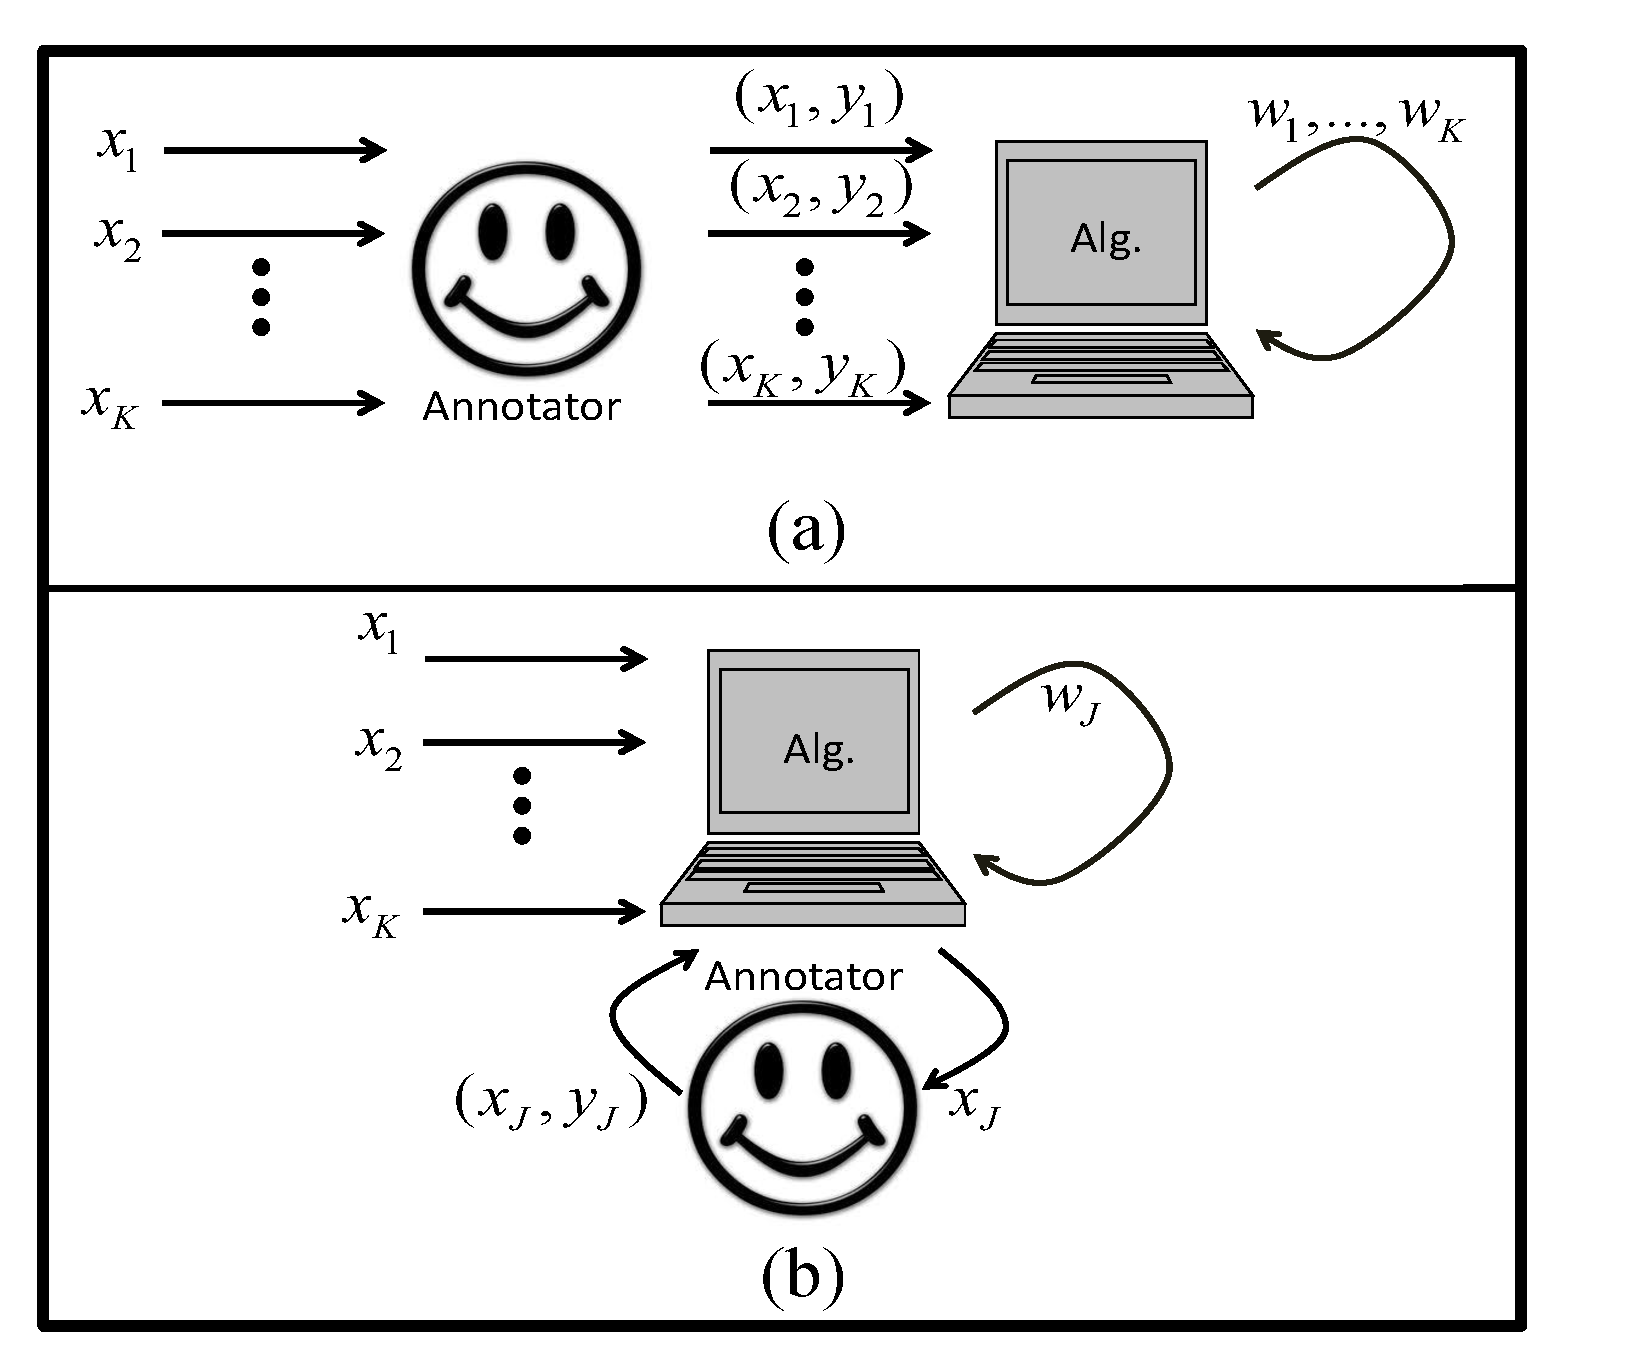
\includegraphics[width=0.7\textwidth]{figs/SHAMPO_illustration.eps}
\end{center}
\end{frame}

\subsection{Related work}

\begin{frame}{ Related Work on multitask learning}

\begin{itemize}
\item \ [Evgeniou et al., 2004] - Tasks comes from same distribution\\
\item \ [Argyriou et al., 2008] - Tasks share small set of features\\
\item \ [Daume et al., 2010] -  Domain adaptation where source and destination share sub hypothesys
\item And more...
\end{itemize}

 All assume relation between  tasks

\end{frame}

\begin{frame}{Selective Sampling}
\textbf{Problem} \newline
\begin{itemize}
\item Labeling  is  expensive - consume resources (time, money, etc.) \newline
\end{itemize}
\textbf{Solution} \newline
\begin{itemize}
\item Only some  labels are queried, others remain unknown\newline
\item Two questions: When should we query? How to update?\newline
\end{itemize}

In our problem, the question \textcolor{red}{"when"}, becomes \textcolor{red}{"which task}"\newline

[Cesa-Bianchi et al., 2006, 2009], [Dekel et al., 2010] ,\newline
[Crammer , 2014] \newline
\end{frame}

\begin{frame}{Selective sampling-example}
Parallel selective sampling setting:
\begin{center}
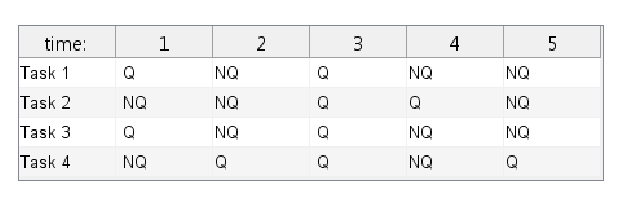
\includegraphics[width=0.6\textwidth]{figs/Table_ss.eps}
\end{center}
Our setting:
\begin{center}
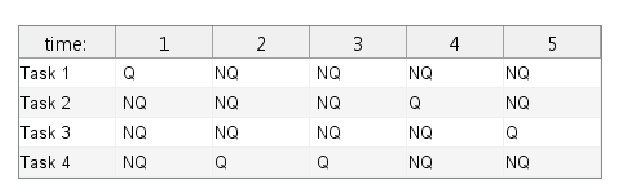
\includegraphics[width=0.6\textwidth]{figs/Table_shampo.eps}
\end{center}
Q=Queried,   NQ=Not Queried
\end{frame}

\subsection{Work guidelines}

\begin{frame}{In this work}
\begin{itemize}
\item Propose  ways for feedback selection (to answer the question "which task?").   \newline
\item Devise    \textcolor{red}{SHAMPO} algorithms  - SHared Annotator for Multiple PrOblems\newline
\item Analyze -  mistakes bound \newline
\item Empirical study that strengthen the algorithms\newline
\end{itemize}
\end{frame}


\begin{frame}{Feedback selection - guidelines}
How to issue a query?\newline
\begin{itemize}
\item Ask when  wrong prediction is assumed\newline
\item Two possible ways:\newline
\begin{itemize}
\item Similarity to previous  labeled  examples \newline
\item Prediction is not distinctive\end{itemize}
\end{itemize}
\end{frame}

\section{First Order Algorithms}

\begin{frame}{Problem Setting}
Problem setup:\newline
\begin{itemize}
\item $K$ binary tasks to be learned \newline
\item $\vxi{i,t}\in \reals^{d_i}$,~~~$i\in\braces{1,\cdots,K}$, - instance vector\newline
\item $y_{i,t}\in\{\pm1\}$ - label\newline
\end{itemize}


\end{frame}

\subsection{Perceptron SHAMPO}

\begin{frame}{Perceptron SHAMPO  - definitions}
\begin{itemize}
\item Linear classifier $\vwi{i,t}\in \reals^d$ \newline
\item Margin $\hat{p}_{i,t}=\vwti{i,t-1}\vxiit $\newline
\item Predicted label $\hyi{i,t}=\sign(\hat{p}_{i,t})$\newline
\item Mistake indicator $M_{i,t}=\mathbb{I}\brackets{\hyi{i,t}\ne y_{i,t}}\in\braces{0,1}$\newline
\item Query  indicator $Z_{i,t}\in\braces{0,1}$\newline
\begin{itemize}
\item $\sum_{i=1}^{K} Z_{i,t}=1 ~~,\forall t$\newline
\end{itemize}
\end{itemize}
\end{frame}


\begin{frame}{Perceptron SHAMPO }
Margin can measure certainty \newline
\begin{itemize}
\item large $\abs{\hat{p}_{i,t}}\Rightarrow$ high certainty\newline
\item small $\abs{\hat{p}_{i,t}}\Rightarrow$ low certainty
\end{itemize}
\begin{center}
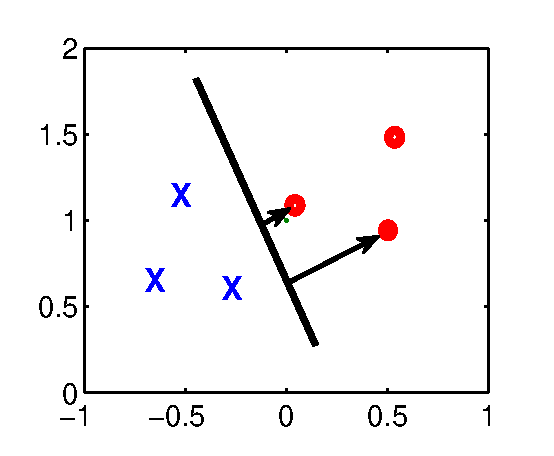
\includegraphics[width=0.5\textwidth]{figs/margin.eps}
\end{center}
\end{frame}

\begin{frame}{perceptron SHAMPO }
Define $J_t$ - the chosen task in time $t$\newline

The probability to query the task $j\in\braces{1\cdots,K}$ is:\newline
\begin{equation*}
\begin{aligned}
 \pr{J_t=j}&=\frac{1}{D_t}\frac{1}{\paren{b+\textcolor{red}{\abs{\hat{p}_{j,t}}-\min_{m=1}^K\abs{\hat{p}_{m,t}}}}} ~~\forall j\in\braces{1\cdots,K}\\
~ \textrm{ for }~
D_{t}&=\sum_{i=1}^{K}{\paren{b+\abs{\hat{p}_{i,t}}-\min_{m}\abs{\hat{p}_{m,t}}}^{-1}},~~~  b>0\in\reals
\end{aligned}
\end{equation*}
\begin{itemize}
\item Large $b \paren{b >> 1}\Rightarrow$ uniform distribution - exploration \newline
\item Small $b\paren{b\rightarrow 0 } \Rightarrow$ delta distribution - exploitation\newline
\item The data need to be  scaled into a ball, e.g. $\normt{\vxi{i,t}}\le1$ 
\end{itemize}
\end{frame}

\begin{frame}{ Probability example}
Example of the distribution over 2 tasks.\newline

Fix $\abs{\hat{p}_{2,t^*}}=0.5$\newline

The probability to choose task 1 is:
\begin{center}
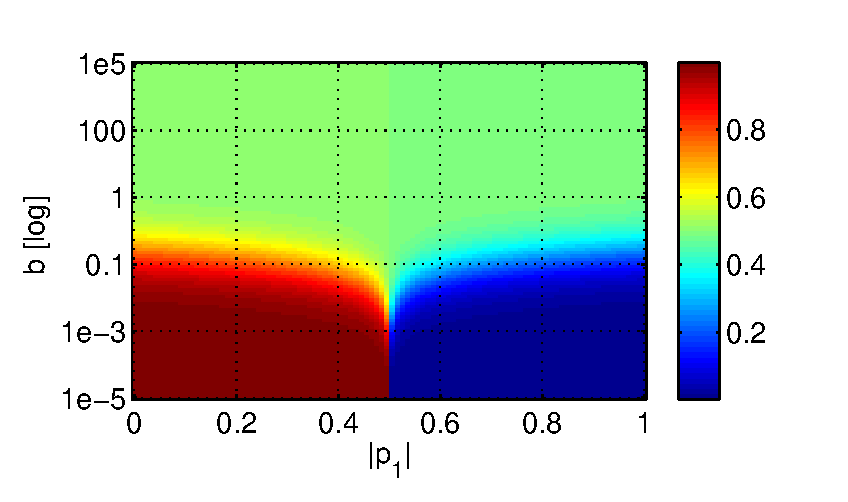
\includegraphics[width=0.60\textwidth]{figs/probability.eps}
\end{center}
\end{frame}

\begin{frame}{perceptron SHAMPO - probability}
Advantages of   random selection:\newline
\begin{itemize}
\item A few tasks has  similar  margin\newline
\item To cope with adversary\newline
\item To get  exploration-exploitation
\end{itemize}
\end{frame}

\begin{frame}{perceptron SHAMPO }
Initialize: $\vwi{i,0}=\vzero$, $b\in\mathbb{R}>0$\newline

On each round $t$, the algorithm: \newline
\begin{itemize}
\item Observes $K$ instances $\vxi{i,t}$  \newline
\item Predicts $K$ labels  $\hat{y}_{i,t}=\sign{(\vwti{i,t-1} \vxiit)}$ \newline
\item Chooses a task to query  with probability  $\pr{J_t=j}$  \newline
\item Query the label $y_{J_t,t}$ \newline
\item Sets $M_{J_t}=1$ ~~~~ iff~~~~ $\hat{y}_{J_t,t}\ne y_{J_t,t}$\newline
\item Updates :~~~~
$\vwi{J_t,t} =\vwi{J_t,t-1}+M_{J_t,t} \,\yi{J_t,t}\, \vxi{J_t,t}$
\end{itemize}
\end{frame}




\subsection{Aggressive perceptron SHAMPO}

\begin{frame}{Aggressive perceptron SHAMPO  }
\begin{itemize}
\item Aggressive update: correct prediction but low margin.\newline
\item $\lambda\in \reals>0$, -  aggressiveness threshold\newline
\item Aggressive update indicator $G_{i,t}=\mathbb{I}\brackets{\abs{\hat{p}_{i,t}}<\lambda,M_{i,t}=0}\in\braces{0,1}$\newline
\item Update  indicator $U_{i,t}=M_{i,t}+G_{i,t}\in\braces{0,1}$\newline
\end{itemize}
\end{frame}


\subsection{SHAMPO with prior}

 \begin{frame}{SHAMPO with prior}

 If we have a prior knowledge about the  tasks, we prefer  to change the distribution to:\newline

 \begin{equation*}
 \pr{J_t=j} =
 \frac{1}{D_{t}}\frac{a_{j}}{\paren{b+\abs{\hat{p}_{j,t}}-\min_{m=1}^K\abs{\hat{p}_{m,t}}}}, \end{equation*}\newline
 with the appropriate normalization factor $D_t$\newline
 \begin{itemize}
 \item The "prior" parameters $a_j\ge1$ (for the analysis)\newline
 \item Large $b\Rightarrow$ prior distribution \newline
 \item Small $b\Rightarrow$ delta distribution\newline
 \end{itemize}
 \end{frame}


\subsection{Mistakes bound}
\begin{frame}{Perceptron SHAMPO  loss}
\begin{itemize}
\item $\vu_i\in\reals^d$ is arbitrary hyperplane \newline
\item Hinge loss function $\lossp{\gamma,i,t}(\vui{i})= \paren{\gamma-\yiit
  \vuti{i}\vxiit}_{+}~,~~\gamma>0$ \newline
\item Expected loss over updates up to time $T$
\begin{equation*}
 \bar{L}_{\gamma,T}=\mathbb{E}\brackets{\sum_{t=1}^T \sum_{i=1}^{K}{Z_{i,t}U_{i,t}\lossp{\gamma,i,t}(\vui{i})}}\newline
\end{equation*}
\item $\tilde{U}^2=\sum_{i=1}^{K}\normt{\vui{i}}$~, ~~ $X=\max_{i,t}\Vert\vxiit\Vert$
\end{itemize}
\end{frame}


%\begin{frame}{Perceptron SHAMPO bound}
%\begin{block}{Expected mistakes bound}
%\emph{The expected number of mistakes  of the perceptron SHAMPO  up to time $T$ can be bounded as follows:}
%\begin{displaymath}
%\mathbb{E}\left[ \sum_{i=1}^{K}\sum_{t=1}^{T}{M_{i,t}} \right]
%\le \frac{K}{\gamma}\left(1+\frac{X^2}{2b} \right){\bar L}_{\gamma,T}
%+\frac{K\left({2b+X^2}\right)^2\tilde{U}^2}{8{\gamma}^2b}~
%\end{displaymath}
%\emph{where}~~~ $\tilde{U}^2=\sum_{i=1}^{K}\normt{\vui{i}}$~, ~~ $X=\max_{i,t}\Vert\vxiit\Vert$
%\end{block}
%\begin{itemize}
%
%\item When $b$ increase, the first term decrease and the second increase and vice versa\newline
%\item Get partial feedback, yet achieves good results
%\end{itemize}
%\end{frame}


\begin{frame}{Perceptron SHAMPO   bound }
\begin{block}{Expected mistakes bound}
\emph{There exist $0<\delta\le\sum_{i=1}^Ka_{i  }$ such that the expected  number of mistakes  of the  perceptron SHAMPO  up to time $T$can be bounded as follows:}
\begin{displaymath}
\begin{split}
\mathbb{E}\left[ \sum_{i=1}^{K}\sum_{t=1}^{T}{M_{i,t}} \right]
\le& \frac{\delta}{\gamma}\brackets{\left(1+\frac{X^2}{2b} \right){\bar L}_{\gamma,T}+
\frac{\left({2b+X^2}\right)^2\tilde{U}^2}{8{\gamma}b}}\\
&\textcolor{red}{-\paren{1-2\frac{\lambda}{b}}\mathbb{E}\brackets{\sum_{i=1}^{K}\sum_{t=1}^{T}{a_iG_{i,t}}}}~
\end{split}
\end{displaymath}
\end{block}
\begin{itemize}
\item A good choice $\lambda<b/2 $\newline
\item When $\lambda\rightarrow0\Longrightarrow\mathbb{E}\brackets{\sum_{i=1}^{K}\sum_{t=1}^{T}{a_iG_{i,t}}}\rightarrow0$
\end{itemize}
\end{frame}

% \begin{frame}{Aggressive perceptron SHAMPO with prior}
% \begin{block}{Expected mistake bound}
% \emph{The  expected number of mistakes of the aggressive perceptron SHAMPO  with prior up to time $T$ can be bounded as follows:}
% \begin{displaymath}
% \begin{split}
% \mathbb{E}\left[ \sum_{i=1}^{K}\sum_{t=1}^{T}{M_{i,t}} \right]
% \le\frac{\textcolor{red}{\paren{\sum_{j=1}^Ka_{j}}}}{\gamma}\brackets{\left(1+\frac{X^2}{2b} \right){\bar L}_{\gamma,T}+
% \frac{\left({2b+X^2}\right)^2\tilde{U}^2}{8{\gamma}b}}\\
% -\paren{1-2\frac{\lambda}{b}}\mathbb{E}\brackets{\sum_{i=1}^{K}\sum_{t=1}^{T}{\textcolor{red}{a_{i}}A_{i,t}}}
% \end{split}
% \end{displaymath}
% \end{block}
% \begin{itemize}
% \item When $a_{i,t}=1~,\forall i=1,\cdots,K$ we get the aggressive bound\newline
% \item When $A_{i,t}=0~,\forall i=1,\cdots,K$ we get the non aggressive bound\newline
% \end{itemize}
%\end{frame}
%
% \begin{frame}
% \begin{table}[h]
% \caption{Bounds} % title name of the table
% \centering % centering table
% \begin{tabular}{l c} % creating 10 columns
% \hline\hline % inserting double-line
% & $\frac{K}{\gamma}\brackets{\left(1+\frac{X^2}{2b} \right){\bar L}_{\gamma,n}+
% \frac{\left({2b+X^2}\right)^2\tilde{U}^2}{8{\gamma}b}}$\\ [-1ex]
% \raisebox{1.5ex}{perceptron}&\\[1ex]
%
% & $\frac{K}{\gamma}\brackets{\left(1+\frac{X^2}{2b} \right){\bar L}_{\gamma,n}+
% \frac{\left({2b+X^2}\right)^2\tilde{U}^2}{8{\gamma}b}}$\\ [-1ex]
% \raisebox{1.5ex}{Aggresive}&$-\paren{1-2\frac{\lambda}{b}}\mathbb{E}\brackets{\sum_{i=1}^{K}\sum_{t=1}^{n}{A_{i,t}}}
% $\\[1ex]
%
% & $\frac{\paren{\sum_{j=1}^Ka_{j}}}{\gamma}\brackets{\left(1+\frac{X^2}{2b} \right){\bar L}_{\gamma,n}+
% \frac{\left({2b+X^2}\right)^2\tilde{U}^2}{8{\gamma}b}}$\\ [-1ex]
% \raisebox{1.5ex}{Prior}&$-\paren{1-2\frac{\lambda}{b}}\mathbb{E}\brackets{\sum_{i=1}^{K}\sum_{t=1}^{n}{a_{i}A_{i,t}}}
% $\\[1ex]
% \hline % inserts single-line
% Entering 1st row
% \hline % inserts single-line
% \end{tabular}
%
% \end{table}
% \end{frame}

% \subsection{Adaptive $b$ SHAMPO}
%
%
 \begin{frame}{SHAMPO with adaptive $b$ }
 \begin{itemize}
 \item How to choose the optimal $b$? ( by experiments - later)\newline

 \item
Task that makes a lot of updates (mistakes) $\longrightarrow$ hard task  \newline
 \end{itemize}
 Define:
 \begin{itemize}
 \item $N_{i,t}$ the number of updates of task $i$ up to time $t$ \newline
 \item  $\tilde{X}_{i,t} = \max\paren{X_{i,t-1},\Vert\vxiit\Vert}$\newline
 \item  $b_{i,t-1}=\beta  \tilde{X}_{i,t}^2\sqrt{N_{i,t-1}+1}$~,~~ $\beta\in\reals>0$
 \begin{align}
 \pr{J_t=j} &=\frac{1}{D_t}\frac{b_{i,t}}{b_{i,t}+\abs{\hat{p}_{j,t}}-\min_{m=1}^K\abs{\hat{p}_{m,t}}},\nonumber\\
D_t &=\sum_i \frac{b_{i,t}}{b_{i,t}+\abs{\hat{p}_{j,t}}-\min_{m=1}^K\abs{\hat{p}_{m,t}}}
 \end{align}
 \end{itemize}
 \end{frame}


 \begin{frame}{SHAMPO with adaptive $b$}
 \begin{block}{Expected Mistake bound}
  \emph{There exist $0<\delta\le K$ such that the expected  number of mistakes  of the  adaptive 
  perceptron SHAMPO  up to time $T$can be bounded as follows:}
% The  expected number of mistakes number of the adaptive $b$ perceptron SHAMPO  can be bounded as follows:
 \begin{displaymath}
\mathbb{E}\brackets{ \sum_{i=1}^{K}\sum_{t=1}^{T}{M_{i,t}}}
\le \delta\brackets{\frac{\delta B^2}{2}+\frac{1}{\gamma}{\bar L}_{\gamma,T}+\frac{KR}{2\beta}
+ B\sqrt{\frac{\delta B^2}{4}+\frac{1}{\gamma}{\bar L}_{\gamma,T}+\frac{KR}{2\beta}}}
 \end{displaymath}
 Where $R = \max_i{\paren{\Vert u_i\Vert X_i}/{\gamma}}$, $B=\paren{R+\frac{2+3R}{2\beta}}$ 
 \end{block}
 \begin{itemize}
 \item Doesn't consider the queries\newline
 \item Suggestion: instead $\sqrt{N_{i,t-1}+1}$, ~~~use $\sqrt{(N_{i,t-1}+1)/(\sum_t{Z_{i,t}}})$  \newline
 \end{itemize}
 \end{frame}

\section{Second Order Algorithm}
%
%
% \begin{frame}{Second order SHAMPO}
% So far our measures for hardness of tasks are: \newline
% \begin{itemize}
% \item The margin\newline
% \item Number of queries\newline
% \end{itemize}
% We had not exploit the similarity  of input examples yet.
% \end{frame}

\begin{frame}{Second order SHAMPO}
Adapting the RLS (Regularized Least squares) estimator from regression to binary 
classification,
%\begin{equation*}
%\vwi{i,t}=A_{i,t}^{-1}\vvi{i,t}
%\end{equation*}
where:\newline
\begin{itemize}
\item $A_{i,0}=I_{d\times d}$\newline
\item $A_{i,t}=\paren{A_{i,t-1}+ U_{i,t}Z_{i,t}\vxi{i,t} \vxti{i,t}}\in R^{d\times d}$\newline
\item $\vwi{i,t}=\vwi{i,t-1}+U_{i,t}Z_{i,t}y_{i_t}\vxi{i,t}\in R^d$ \newline
\end{itemize}
$A_t$ can be viewed as covariance or "confidence " matrix\newline

 [Cesa-Bianchi et al. 2006, Crammer  2014]
\end{frame}

\begin{frame}{Second order SHAMPO}
Initialize: $\vwi_{i,0}$$= \vzero$, $A_{0}=I,~~b\in\mathbb{R}>0$\newline

On each round $t$ \newline
\begin{itemize}
\item Observe $K$ instances $\vxi{i,t}$ \newline
\item Compute  $K$ margins  $\hat{p}_{i,t}= \vxiit^T\paren{A_{i,t-1}+\vxiit\vxiit^T}^{-1}\vw_{i,t-1}$\newline
\item Predict $K$ labels $\hat{y}_{i,t}=\sign\paren{\hat{p}_{i,t}}$\newline
\item Query the label $y_{J_t,t}$ with same probability  $\pr{J_t=j}$ as in first order \newline
\item Update :~~~~
$\vw_{J_t,t}~~,~~ A_{J_t,t} $\newline
\end{itemize}
\end{frame}

\begin{frame}{Second order SHAMPO}
\begin{block}{Expected mistake bound}
\emph{There exists $0<\delta\le K$, such that the  expected number of mistakes  of the second order perceptron SHAMPO  up to time $T$ can be bounded as follows:}
  \begin{equation*}
  \begin{split}
   &\mathbb{E}\brackets{\sum_{i=1}^{K}\sum_{t=1}^{T}{M_{i,t}}} \\
   &\le \frac{\delta}{\gamma}{\bar L}_{\gamma,T}(\vui{i})
+ \frac{\delta b}{2\gamma^2}\sum_{i=1}^{K}\vu_i^T\mathbb{E}\brackets{A_{i,T}}\vu_i+ 
\frac{\delta}{2b}\sum_{i=1}^{K}\sum_{k=1}^{d}\mathbb{E}\brackets{\ln\paren{1+\lambda_{i,k}}}
\end{split}
\end{equation*} 
\end{block}

\begin{itemize}
  \item  $\lambda_{i,k}$ is an $i^th$ eigenvalue of the matrix $A_{i,T}$
\end{itemize}

\end{frame}

\begin{frame}{Second order SHAMPO - Aggressive}
This is the state in time $t$
\begin{center}
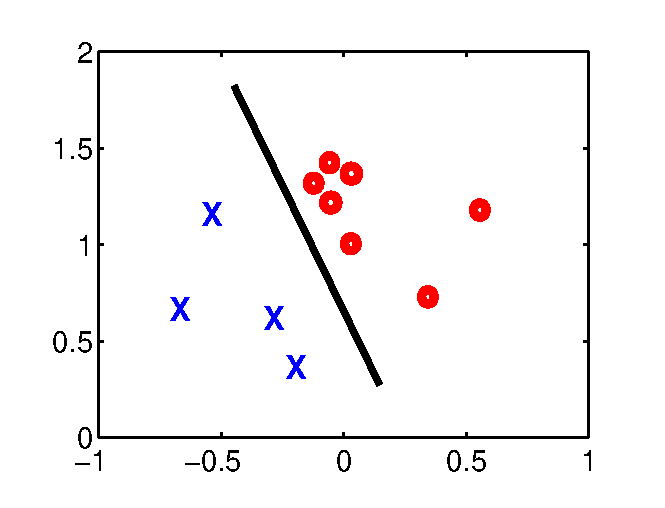
\includegraphics[width=0.7\textwidth]{figs/confidence.eps}
\end{center}
\end{frame}

\begin{frame}{Second order SHAMPO - Aggressive}
On $t+1$ we get a new example (black square). What will be it's label?
\begin{center}
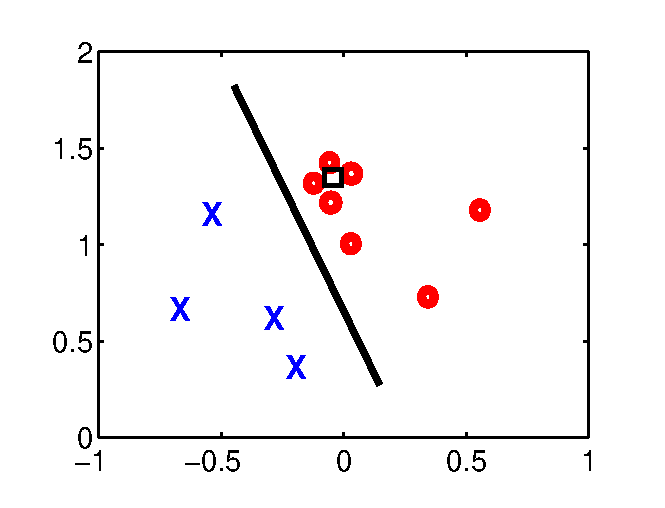
\includegraphics[width=0.7\textwidth]{figs/confidence2.eps}
\end{center}
\end{frame}

\begin{frame}{Second order SHAMPO - Aggressive}
Define $r_{i,t}= \vxiit^TA_{i,t-1}^{-1}\vxiit$  \newline
\begin{itemize}
\item $r_{i,t}$ - the confidence  in the prediction of $\hat{y}_{i,t}$\newline
%\item $r_{i,t}$ does not depend explicitly on the  feedback \newline
\item Large $r_{i,t}\Rightarrow$ low confidence \newline
\item Small $r_{i,t}\Rightarrow$ high confidence \newline
\item If $\normt{\vxi{i,t}}\le1, \forall i,t$ then $0<r_{i,t}\le1$
\end{itemize}
\end{frame}

%\begin{frame}{Second order SHAMPO}
%An intuition for the confidence $r_{i,t}$
%\begin{center}
%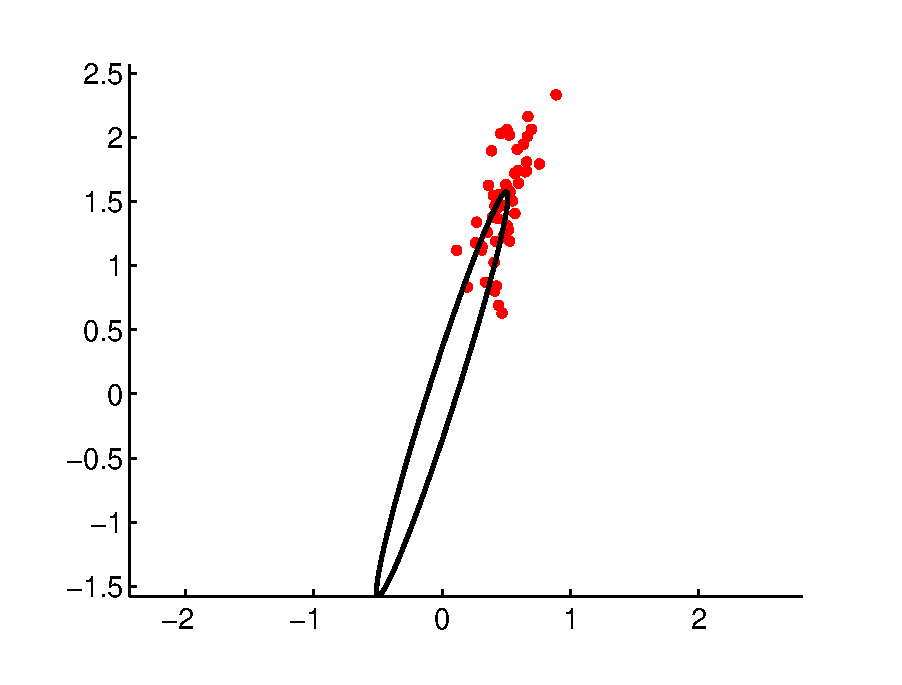
\includegraphics[width=0.6\textwidth]{figs/Confidence_matrix.eps}
%\end{center}
%\end{frame}

\begin{frame}{Second order SHAMPO - Aggressive}
Define:
\begin{equation*}
F\paren{\abs{\hat{p}_{i,t}},r_{i,t}}=\paren{1+r_{i,t}}\hat{p}_{i,t}^2+2\abs{\hat{p}_{i,t}}-\frac{r_{i,t}}{1+r_{i,t}}\newline
\end{equation*}
We build a new distribution:
\begin{equation*}
\begin{aligned}
\pr{J_t=j}&=\frac{1}{D_t}\frac{1}{\paren{b+F\paren{\abs{\hat{p}_{i,t}},r_{i,t}}_{+}}} ~~\forall j\in\braces{1\cdots,K}\\
 ~ \textrm{ Where }~
 D_{t}&=\sum_{i=1}^{K}{\paren{b+F\paren{\abs{\hat{p}_{i,t}},r_{i,t}}_{+}}^{-1}}
\end{aligned}
\end{equation*}

\begin{itemize}
\item $F\paren{\abs{\hat{p}_{i,t}},r_{i,t}}\le0$  ~~iff~~ $\abs{\hat{p}_{i,t}}\le\frac{-1+\sqrt{1+r_{i,t}}}{1+r_{i,t}}\le\frac{-1+\sqrt{2}}{2}\approx0.2 $  (aggressive)\newline
\end{itemize}
\end{frame}

\begin{frame}{Second order SHAMPO - Aggressive - $F\paren{\abs{\hat{p}_{i,t}},r_{i,t}}$}
\begin{figure}
\begin{centering}
\includegraphics[width=0.65\textwidth]{figs/theta_plot.eps}
\end{centering}
\end{figure}
\end{frame}

\begin{frame}{Second order SHAMPO - Aggressive}
Initialize: $\vwi_{i,0}$$ =\vzero$, $A_{0}=I,~~b\in\mathbb{R}>0$\newline

On each round $t$ \newline
\begin{itemize}
\item Observe $K$ instances $\vxi{i,t}$ \newline
\item Compute  $K$ margins  $\hat{p}_{i,t}= \vxiit^T\paren{A_{i,t-1}+\vxiit\vxiit^T}^{-1}\vw_{i,t-1}$\newline
\item Predict $K$ labels $\hat{y}_{i,t}=\sign\paren{\hat{p}_{i,t}}$\newline
\item Query the label $y_{J_t,t}$ with probability  $\pr{J_t=j}$ above, \newline
\item If $F\paren{\abs{\hat{p}_{J_t,t}},r_{J_t,t}}\le0$ or $\hat{y}_{J_t,t}\ne y_{J_t,t}$ set $U_{J_t,t}=1$\newline
\item Update :~~~~
$\vw_{J_t,t}~~,~~ A_{J_t,t}$ iff $U_{iJ_tt}=1$\newline
\end{itemize}
\end{frame}

\section{Variants}

\begin{frame}{Contextual Bandits - decoupling of exploration and exploitation}
The problem: predicting a label $\hat{Y}_t \in\{ 1 \comdots C\}$ given an input $\vxi{t}$\newline
\begin{itemize}
\item Tasks are related\newline
\item Query a single binary question and update the model\newline
\end{itemize}
We consider  two forms  :\newline
\begin{itemize}
\item One vs. one \newline
\item One vs. rest \newline
\end{itemize}
[Kakade et al., 2008], [Hazan et al. 2012]
\end{frame}


\begin{frame}{One vs. rest}

\begin{itemize}
\item There are $K= C$ binary tasks\newline
\end{itemize}
On each round $t$:\newline
\begin{itemize}
\item Observe a single input $\vxii$ \newline
\item Compute $K$  margins $\hat{p}_{i,t}$ for binary tasks \newline
\item Predict the multiclass label, $\hat{Y}_t = \arg\max_i \hat{p}_{i,t}$\newline
\item Choose the label (task) to query on $\bar{Y}_t=J_t$ \newline
\item Update %s the model\newline
\end{itemize}
\end{frame}

\begin{frame}{One vs. rest}
\begin{block}{Expected mistake bound}
There exists $0<\delta\le \sum_{i=1}^Ca_{i}$ such that the  expected number of mistakes  of the One vs. Rest contextual SHAMPO bandit  can be bounded as:

 \[
 \begin{split}
 &\mathbb{E}\brackets{\sum_t \1{Y_t \neq \hat{Y}_t}}\\
 &\le \frac{\delta}{\gamma}\brackets{\left(1+\frac{X^2}{2b} \right){\bar L}_{\gamma,T}+
 \frac{\left({2b+X^2}\right)^2\tilde{U}^2}{8{\gamma}b}}
 +\paren{2\frac{\lambda}{b}-1}\mathbb{E}\brackets{\sum_{i=1}^{K}\sum_{t=1}^{T}{a_{i}G_{i,t}}}~,
 \end{split}
 \]
\end{block}

\begin{itemize}
\item This bound comes from $\mathbb{I}\brackets{Y_t \neq \hat{Y}_t}\le \sum_iM_{i,t}$\newline

\end{itemize}
\end{frame}


\begin{frame}{One vs. one}
\begin{itemize}

\item There are $K= {C\choose2}$ binary tasks.\newline

\end{itemize}
At each round, the algorithm:\newline
\begin{itemize}
\item Gets a single input $\vxii$\newline
\item Computes $K$ predictions  $\hat{y}_{i,t}$ for binary tasks\newline
\item Predicts the multiclass label $\hat{Y}_t$, by tournament. \newline
\item Chooses pair of labels  (task) to  query on $\braces{\bar{Y}_t^{+},\bar{Y}_t^{-}}$ assigned with $J_t$ \newline
\item Update
\end{itemize}
\end{frame}

\begin{frame}{One vs. One}
\begin{block}{Expected mistake bound}
There exists $0<\delta\le \sum_{i=1}^{C \choose 2}a_{i}$ such that the  expected number of mistakes  of the One vs. One contextual SHAMPO bandit  is:
 \[
 \begin{split}
 &\mathbb{E}\brackets{\sum_t \1{Y_t \neq \hat{Y}_t}}\le \frac{2}{({C \choose 2}-1)/2+1}\times\\
 &\braces{ \frac{\delta}{\gamma}\brackets{\paren{1+\frac{X^2}{2b} }{\bar L}_{\gamma,T}+\frac{\paren{{2b+X^2}}^2\tilde{U}^{2}}{8{\gamma}b}}+\paren{2\frac{\lambda}{b}-1}\mathbb{E}\brackets{\sum_{i=1}^{K}\sum_{t=1}^{T}{a_{i}G_{i,t}}}}
 \end{split}
 \]
\end{block}
\begin{itemize}

\item This bound is follows from $\mathbb{I}\brackets{Y_t \neq \hat{Y}_t} \leq \frac{2}{({C \choose 2}-1)/2+1}\sum_{i=1}^{ {C \choose 2}} M_{i,t}$\newline [Allwein et al., 2000]\newline
\item The bound coefficient is upper bounded by 4.
\end{itemize}
\end{frame}

\begin{frame}{One vs. One}
What if the prediction is not a mistake, nor correct , i.e.$y_{J_t,t}=0$?\newline
\begin{itemize}
\item No update -  this task will be chosen again\newline
\item Random update - not allow zero feedback (only $-1$ or $1$)\newline
\item Weak update - increases the margin using $\eta>0$\newline

$
\vwi{J_t,t} = \vwi{J_t,t-1}+ \mathbb{I}\brackets{\yi{J_t,t}\ne0} \, \yi{J_t,t}\, \vxi{J_t,t} +
 \mathbb{I}\brackets{\yi{J_t,t}=0} \eta \hyi{J_t,t}\vxi{J_t,t}~$
\newline
\end{itemize}
%\begin{equation*}
%\begin {aligned}
%\vert \vwti{J_t,t} \vxi{J_t,t} \vert &= \vert
%(\vwi{J_t,t-1}+ \eta \hyi{J_t,t}\vxi{J_t,t})^\top\vxi{J_t,t}\vert \\
%&= \vert \vwti{J_t,t-1}\vxi{J_t,t}+ \eta \sign(\vwti{J_t,t-1}\vxi{J_t,t}) \Vert\vxi{J_t,t}\Vert^2 \vert \\
%&= \vert \vwti{J_t,t-1}\vxi{J_t,t}\vert + \eta \Vert\vxi{J_t,t}\Vert^2 > \vert \vwti{J_t,t-1}\vxi{J_t,t}\vert
%\end{aligned}
%\end{equation*}
\end{frame}

% \begin{frame}{Perceptron SHAMPO for $\kappa$ queries}
% In the case where  we can annotate $\kappa$ tasks in parallel\newline
% \begin{block}{Mistake bound}
% The bound of the expected number of mistakes  of the perceptron SHAMPO with $\kappa$ feedbacks is:
% \begin{displaymath}
% \mathbb{E}\left[ \sum_{i=1}^{K}\sum_{t=1}^{n}{M_{i,t}} \right]
% \le \frac{1}{C(\kappa,K)}\paren{\frac{1}{\gamma}\left(1+\frac{X^2}{2b} \right){\bar L}^\kappa_{\gamma,n}
% +\kappa\frac{\left({2b+X^2}\right)^2}{8{\gamma}^2b}\tilde{U}^2}~
% \end{displaymath}
% \end{block}
% Where
% \begin{itemize}
% \item $C(\kappa,K) = \sum_{j=K-\kappa+1}^{K}\frac{1}{j}$\newline
% \item ${\bar L}^\kappa_{\gamma,n}=\mathbb{E}\brackets{\sum_t^n \sum_{i=1}^{K}{M_{i,t}Z_{i,t}\lossp{\gamma,i,t}(\vui{i})}},$ but now $\sum_{i}Z_{i,t}=\kappa$\newline
% \end{itemize}
% \end{frame}


\section{Experiments}

\begin{frame}{Experiments - Data sets}

\begin{itemize}
\item OCR - USPS \!(7,291 train /2,007 test,$d$=256),\\~~~~~~~~~~
 MNIST\!(60,000 train/10,000 test,$d=784$)  \newline
\begin{itemize}
\item One vs. Rest - 10 tasks\newline
\item One vs. One - 45 tasks \newline
\end{itemize}
\item Vowel prediction - Vocal Joystick (572,911 train /236,680 test, $d=27$)\newline
\begin{itemize}
\item One vs. Rest - 8 tasks\newline
\item One vs. One - 28 tasks \newline
\end{itemize}
\item NLP - sentiment analysis and document classification. - 36 tasks (266,645 examples,\newline
~~ $8,768\le d\le 1,447,866$)\newline
\end{itemize}
\end{frame}

\begin{frame}{Data Subsets collections}
We generated $64$ random sub datasets collection of hard and easy tasks.   
 \begin{table}
\scriptsize   
\begin{tabular}{|l|c|c|c|c|}
\hline
Dataset & \multicolumn{1}{l|}{Max Tasks} & \multicolumn{1}{l|}{Easy group \#} & \multicolumn{1}{l|}{Hard group \#} & \multicolumn{1}{l|}{Collections} \\ \hline
VJ 1 vs 1 & 8 & 10 & 10 & 10 \\ \cline{1-1}
VJ 1 vs Rest & 5 & 4 & 4 & 6 \\ \cline{1-1}
USPS 1 vs 1 & 8 & 20 & 20 & 10 \\ \cline{1-1}
USPS 1 vs Rest & 6 & 5 & 5 & 6 \\ \cline{1-1}
MNIST 1 vs 1 & 8 & 10 & 10 & 10 \\ \cline{1-1}
MNIST 1 vs Rest & 6 & 5 & 5 & 6 \\ \cline{1-1}
NLP documents & 6 & 8 & 8 & 6 \\ \cline{1-1}
MIXED & 8 & 10 & 10 & 10 \\ \hline
\end{tabular}
\end{table}
\end{frame}

\begin{frame}{Data Subsets collections}
All dats subsets are evaluated by two quantities, mean error [\%] 
and mean score (1-6) where 1 is the best (least mean error) .\newline
We also see here that the algorithm works for tasks from different domains (MIXED)
 \begin{table}[h] 
\begin{centering}
{\tiny	
\begin{tabular}{|l|r|r|r|r|r|r|}
\hline
                         & \multicolumn{3}{c|}{\textbf{Aggressive $\lambda=b/2$}}               & \multicolumn{3}{c|}{\textbf{Plain}}                 \\ \hline
\textit{Dataset}         & \textit{exploit} & \textit{SHAMPO}         & \textit{uniform} & \textit{exploit} & \textit{SHAMPO} & \textit{uniform} \\ \hline
{VJ 1 vs 1 }        & 5.22 (2.9)       & \textbf{4.57 (1.1)}   & 5.67 (3.9)       & 5.21 (2.7)       & 6.93 (4.6)    & 6.26 (5.8)       \\
\textrm{VJ 1 vs Rest}    & 13.26 (3.5)      & \textbf{11.73 (1.2)} & 12.43 (2.5)      & 13.11 (3.0)        & 14.17 (5.0)     & 14.71 (5.8)     \\
\textrm{USPS 1 vs 1}      & 3.31 (2.5)       & \textbf{2.73 (1.0)}     & 19.29 (6.0)        & 3.37 (2.5)       & 4.83 (4.0)      & 5.33 (5,0)         \\
\textrm{USPS 1 vs Rest}  & 5.45 (2.8)      & \textbf{4.93 (1.2)}  & 10.12 (6.0)        & 5.31 (2.0)         & 6.51 (4.0)      & 7.06 (5.0)         \\
\textrm{MNIST 1 vs 1}     & 1.08 (2.3)       & \textbf{0.75 (1.0)}     & 5.9 (6.0)         & 1.2 (2.7)       & 1.69 (4.1)      & 1.94 (4.9)     \\
\textrm{MNIST 1 vs Rest} & 4.74 (2.8)      & \textbf{3.88 (1.0)}     & 10.01 (6.0)       & 4.44 (2.8)      & 5.4 (3.8)    & 6.1 (5.0)          \\
\textrm{NLP documents} & 19.43 (2.3)     & \textbf{16.5 (1.0)}     & 23.21 (5.0)        & 19.46 (2.7)     & 21.54 (4.7)  & 21.74 (5.3)     \\
\textrm{MIXED}           & 2.75 (2.4)       & \textbf{2.06 (1.0)}     & 13.59 (6.0)        & 2.78 (2.6)       & 4.2 (4.3)     & 4.45 (4.7)       \\ \hline
\textit{Mean score}      & (2.7)           & \textbf{(1.1)}       & (5.2)           & (2.6)           & (4.3)        & (5.2)           \\ \hline
\end{tabular}
}
\end{centering}
\end{table}
\end{frame}

\begin{frame}{Test Errors of NLP tasks samples}
  Test error of aggressive SHAMPO on four and eight binary text classification tasks. 
\\
Sometime SHAMPO improve not only on cumulative mistakes but also on each individual 
task.
\begin{figure}
\begin{centering}
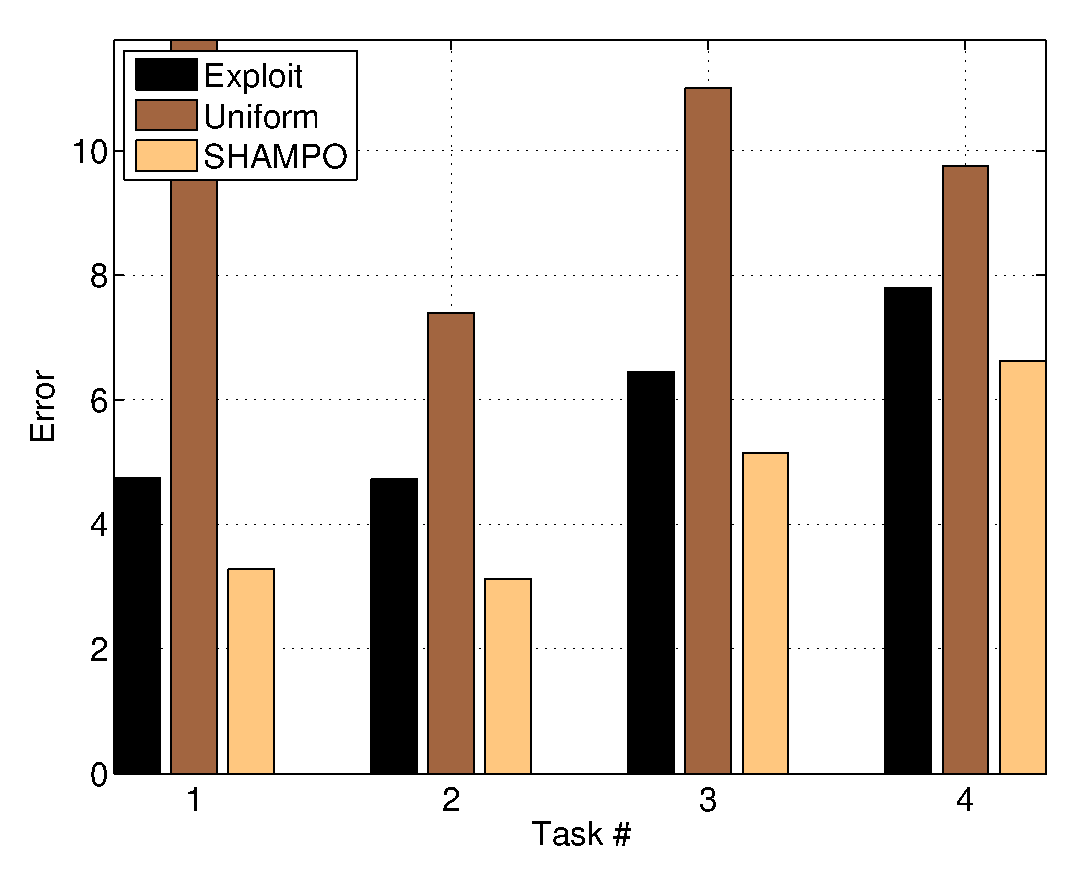
\includegraphics[width=0.45\textwidth]{figs/problem-9_4_2_2-1.eps}
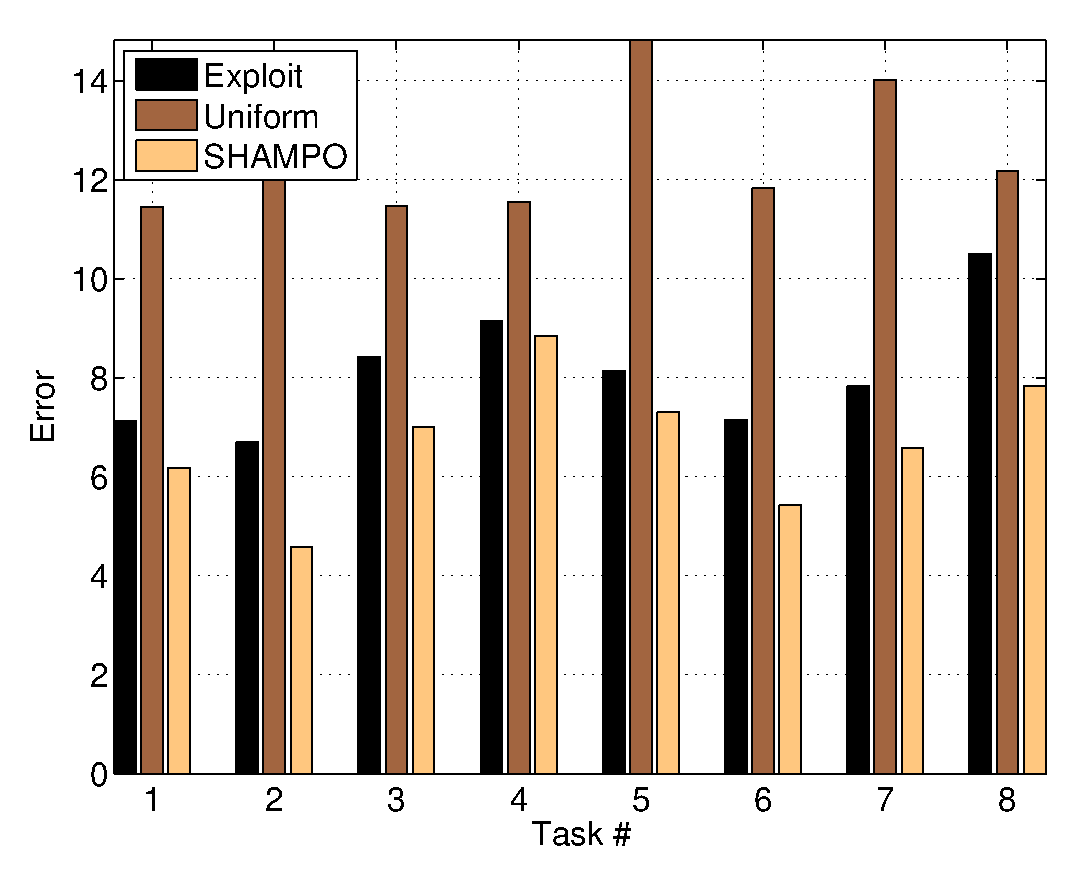
\includegraphics[width=0.45\textwidth]{figs/problem-9_4_4_4-1.eps}
\end{centering}
\end{figure}
\end{frame}

\begin{frame}{One vs. Rest - USPS dataset}
Right values correspond to pure exploration, while left values to pure exploitation.
The only thing we see is the red curve. The "knee" can show the area of the tradeoff $b.$

\begin{figure}
\begin{centering}
\subfigure[Test error ]{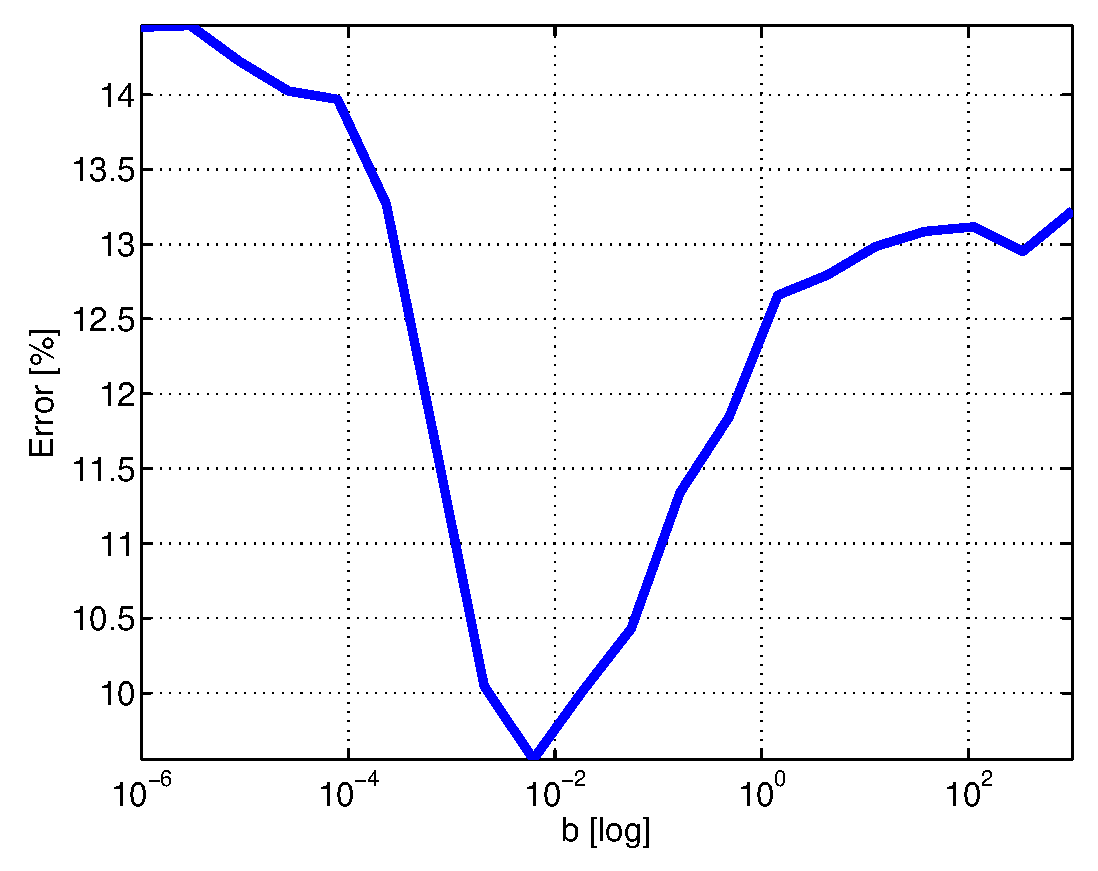
\includegraphics[width=0.45\textwidth]{figs/usps3.eps}}
\subfigure[Train errors ]{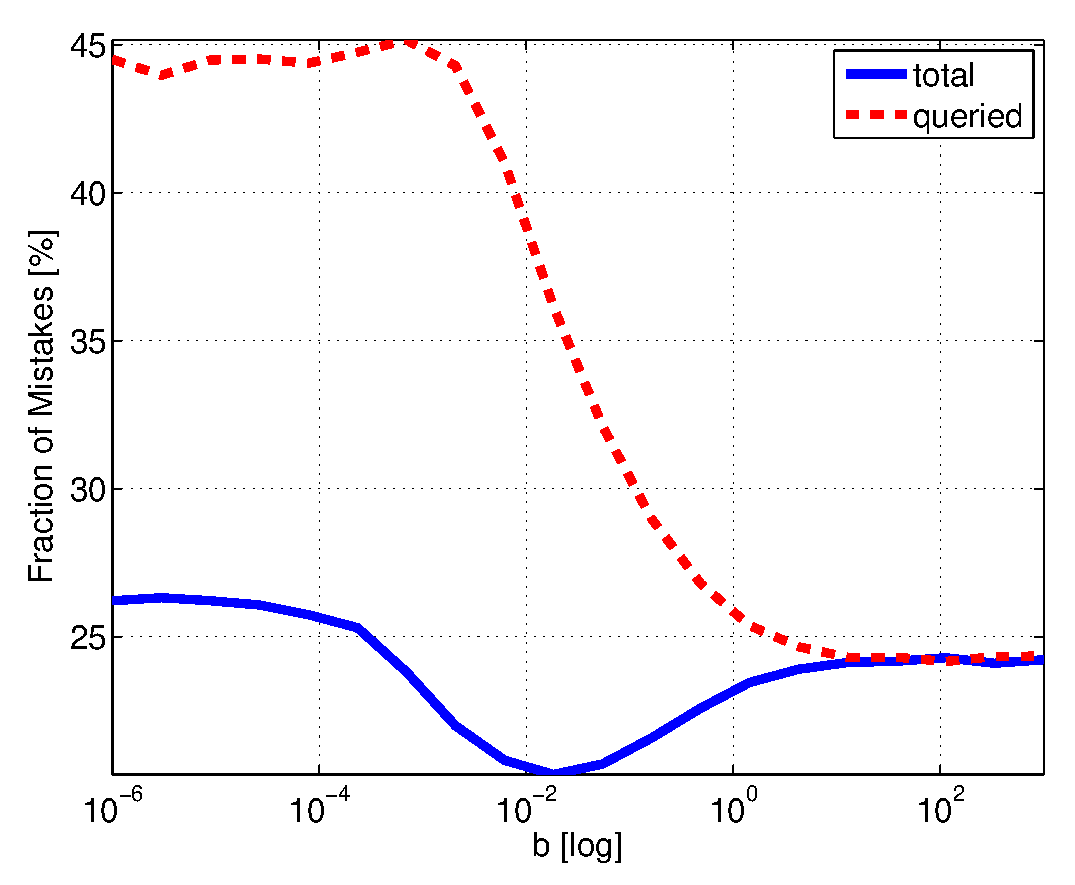
\includegraphics[width=0.45\textwidth]{figs/usps1a.eps}}
%\subfigure[MNIST data]{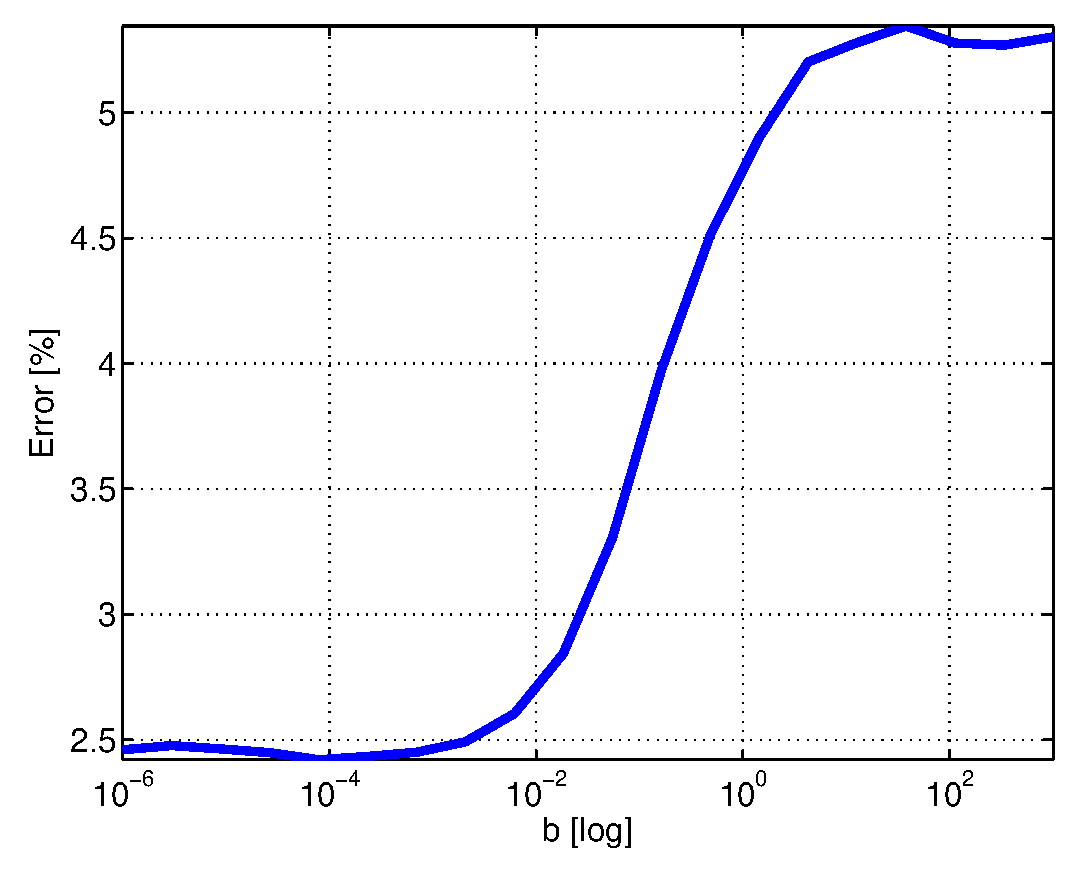
\includegraphics[width=0.32\textwidth]{figs/mnist3.eps}}
%\subfigure[VJ data]{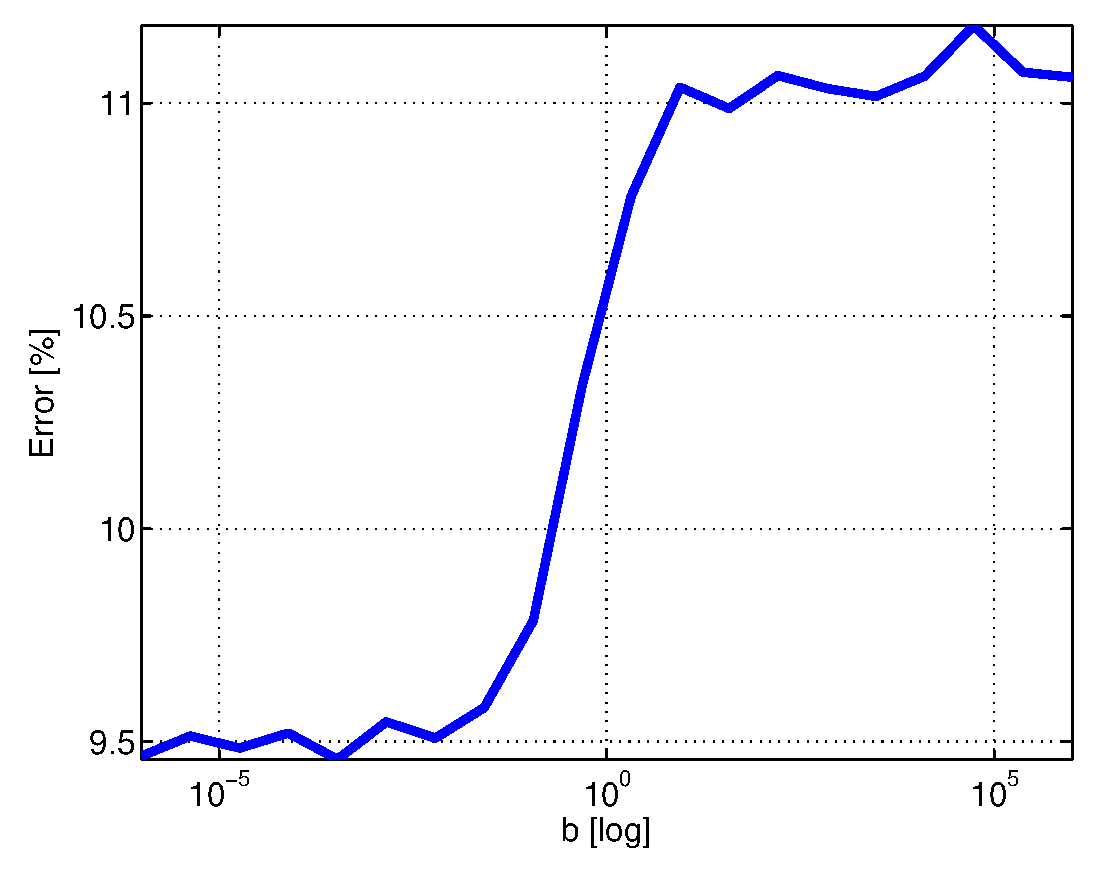
\includegraphics[width=0.32\textwidth]{figs/VJ_pairs3.eps}}
\end{centering}
\end{figure}
\end{frame}

% \begin{frame}{One vs. Rest dataset}
% \textbf{USPS} - One vs. Rest\newline
% The only thing we see is the red curve. The "knee" can show the optimal $b$
%
% % Mean fraction of mistakes during training time, for either only queried inputs (dashed red) or all inputs (blue) vs $b$. High $b$ values indicate pure exploration, and low $b$ values pure exploitation.
% \begin{figure}
% \begin{centering}
% \subfigure[USPS data ]{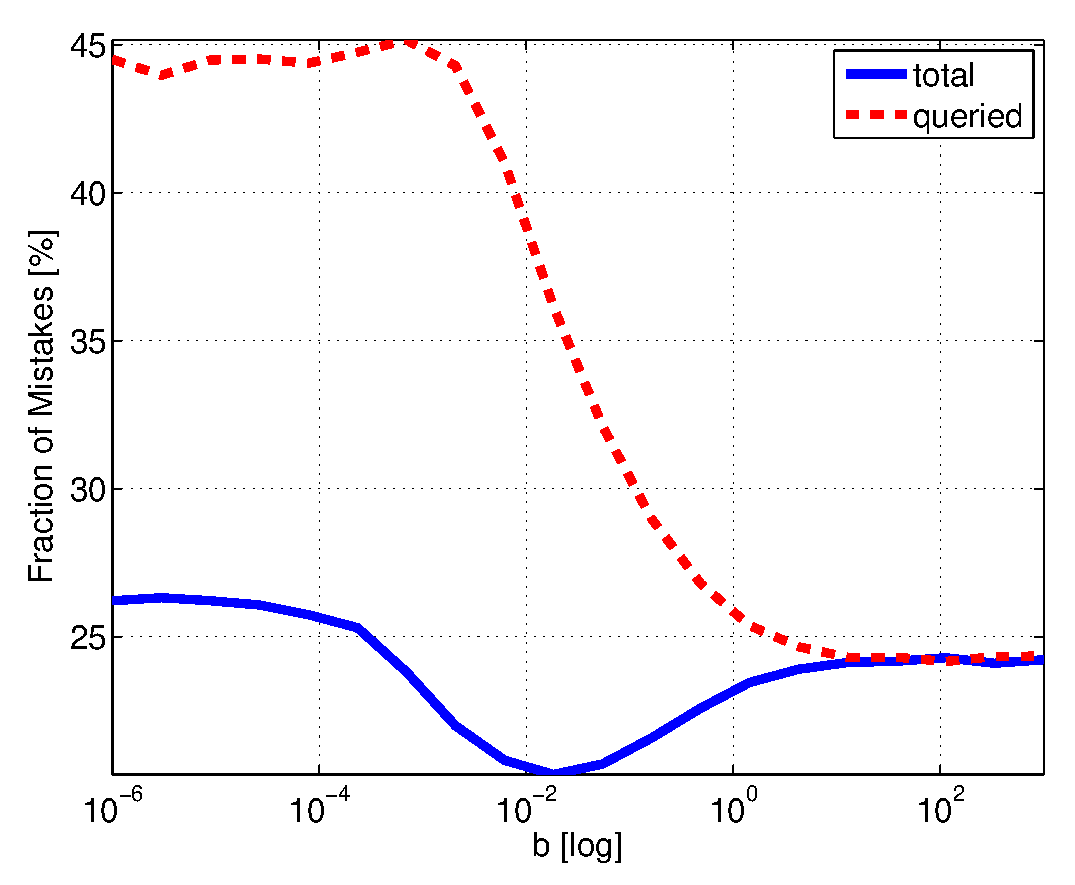
\includegraphics[width=0.32\textwidth]{figs/usps1a.eps}}
% \subfigure[USPS data ]{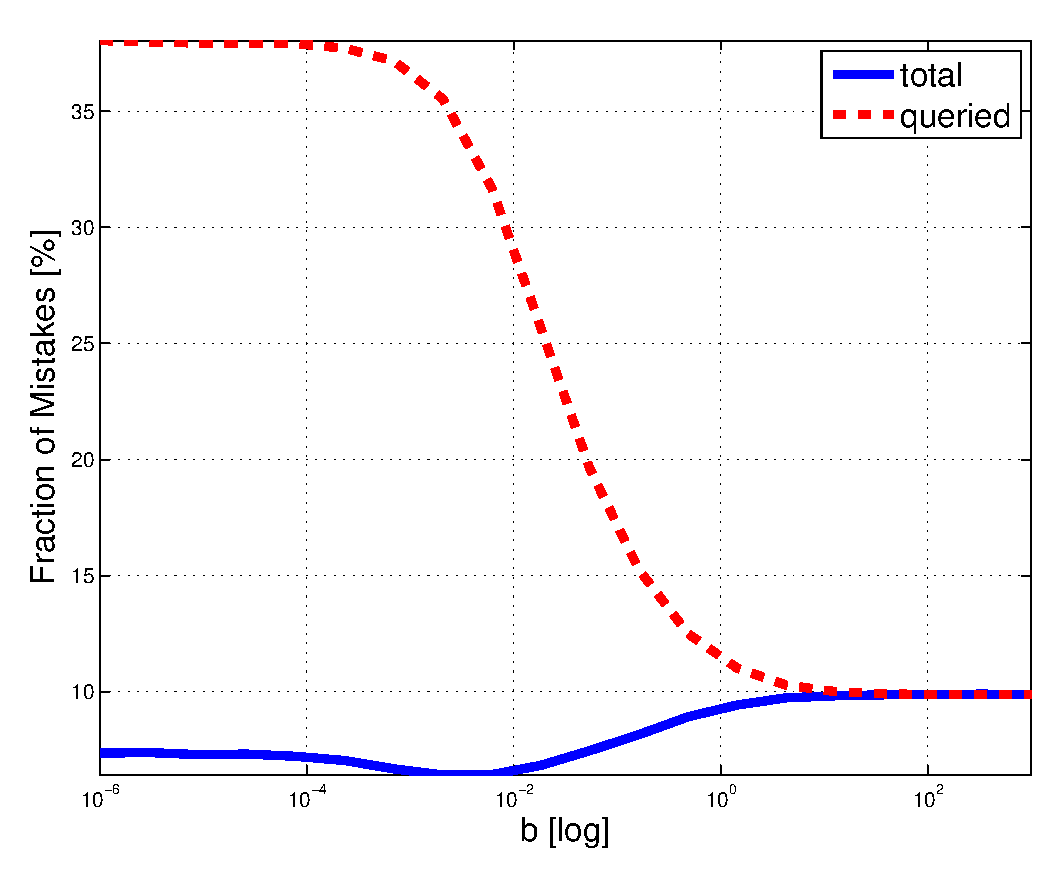
\includegraphics[width=0.32\textwidth]{figs/mnist1a.eps}}
% \subfigure[USPS data ]{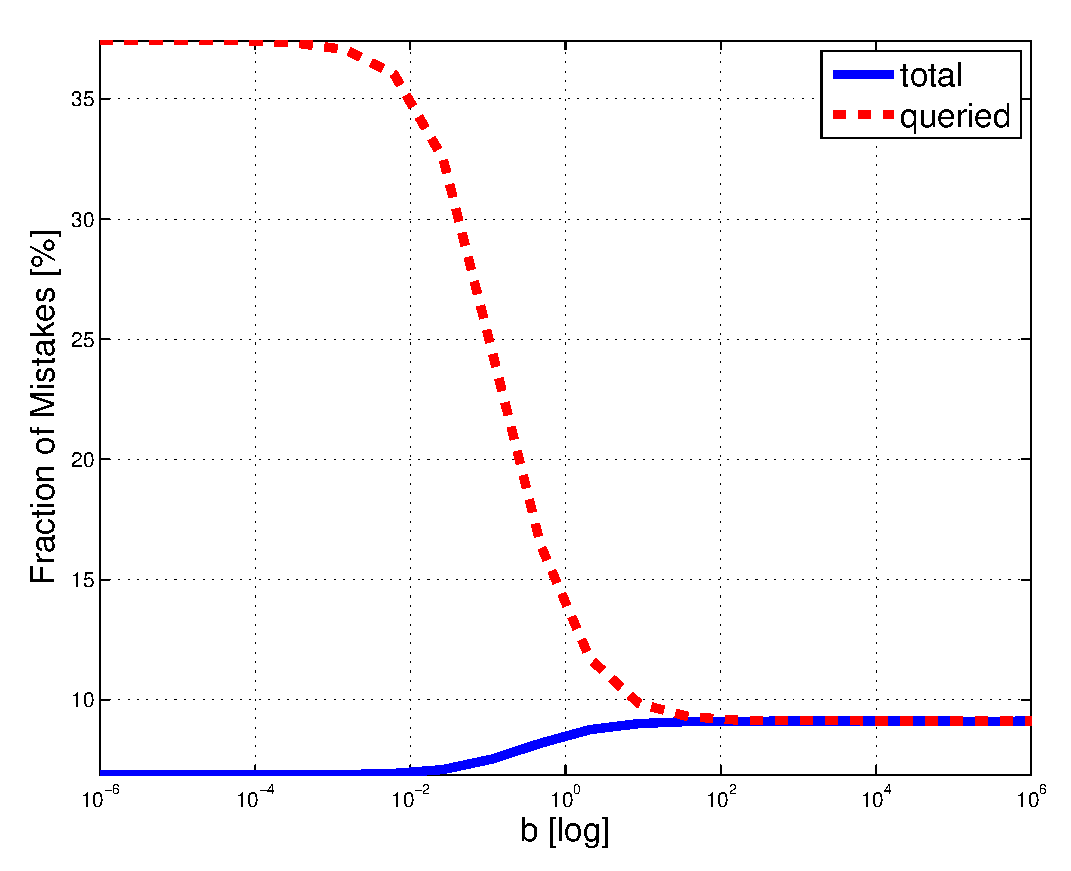
\includegraphics[width=0.32\textwidth]{figs/VJ_pairs1a.eps}}
% \end{centering}
% \end{figure}
%\end{frame}


\begin{frame}{Test error vs. number of queries}
\textbf{MNIST -  One vs. One data} \newline
The tradeoff   shows less errors for the appropriate queries distribution\newline

\begin{centering}
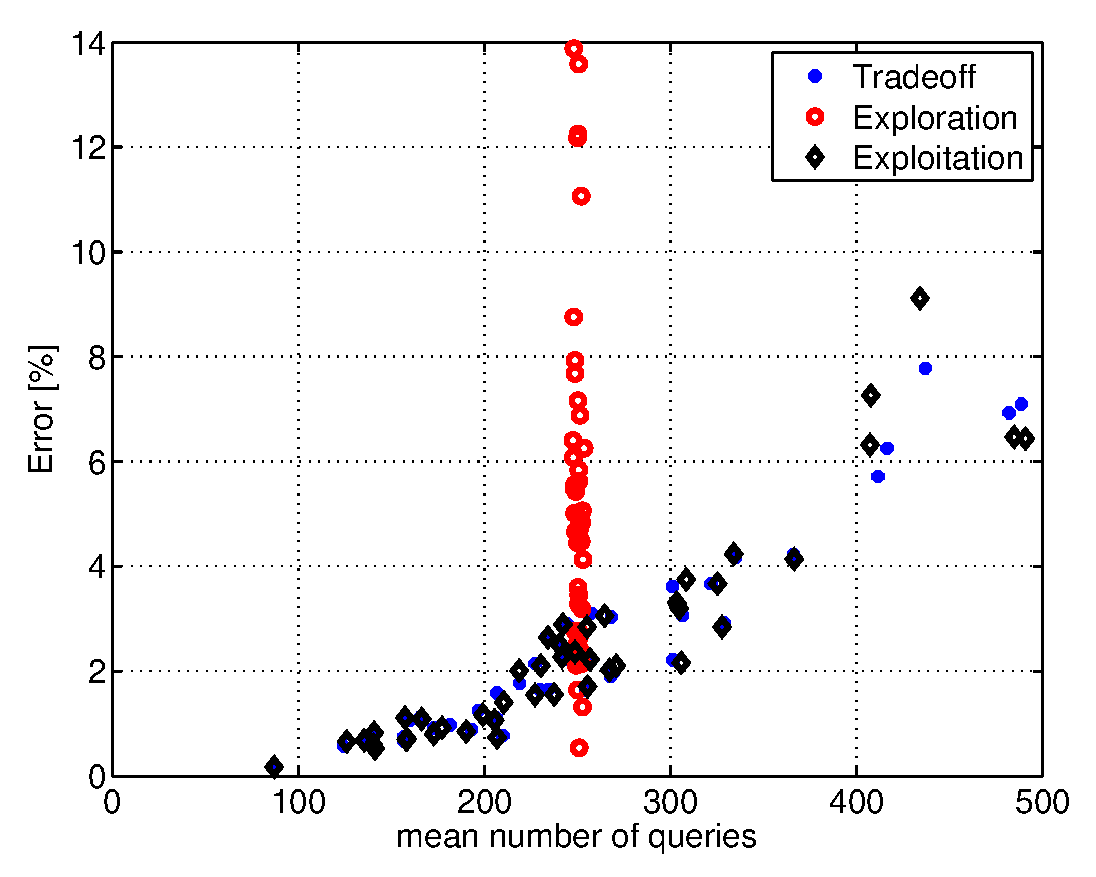
\includegraphics[width=0.6\textwidth]{figs/mnist2b.eps}

\end{centering}

\end{frame}


%\begin{frame}{Error vs. b}
%\textbf{NLP Data - 2 hard tasks, 3 easy, second order} \newline
%Almost all of the tasks shows lower test error for the tradeoff $b$ value  \newline
%
%\begin{centering}
%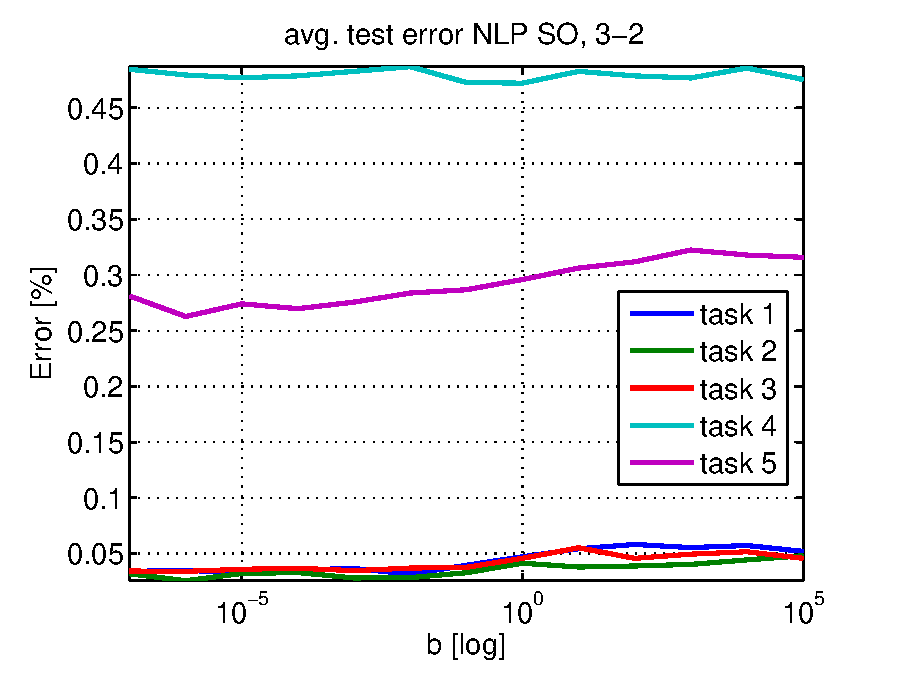
\includegraphics[width=0.6\textwidth]{figs/NLP_SO_3_2_mean_error_tasks.eps}
%
%\end{centering}
%
%\end{frame}



\begin{frame}{Error vs. b - different algorithms (test error) }
\textbf{VJ one-vs-one} \newline
Comparison between different algorithms. 
First Order, Aggressive, Adaptive, Prior, Second order, Second order aggressive and ''Watch All''.
All algorithms show the same behavior.  \newline

\begin{centering}
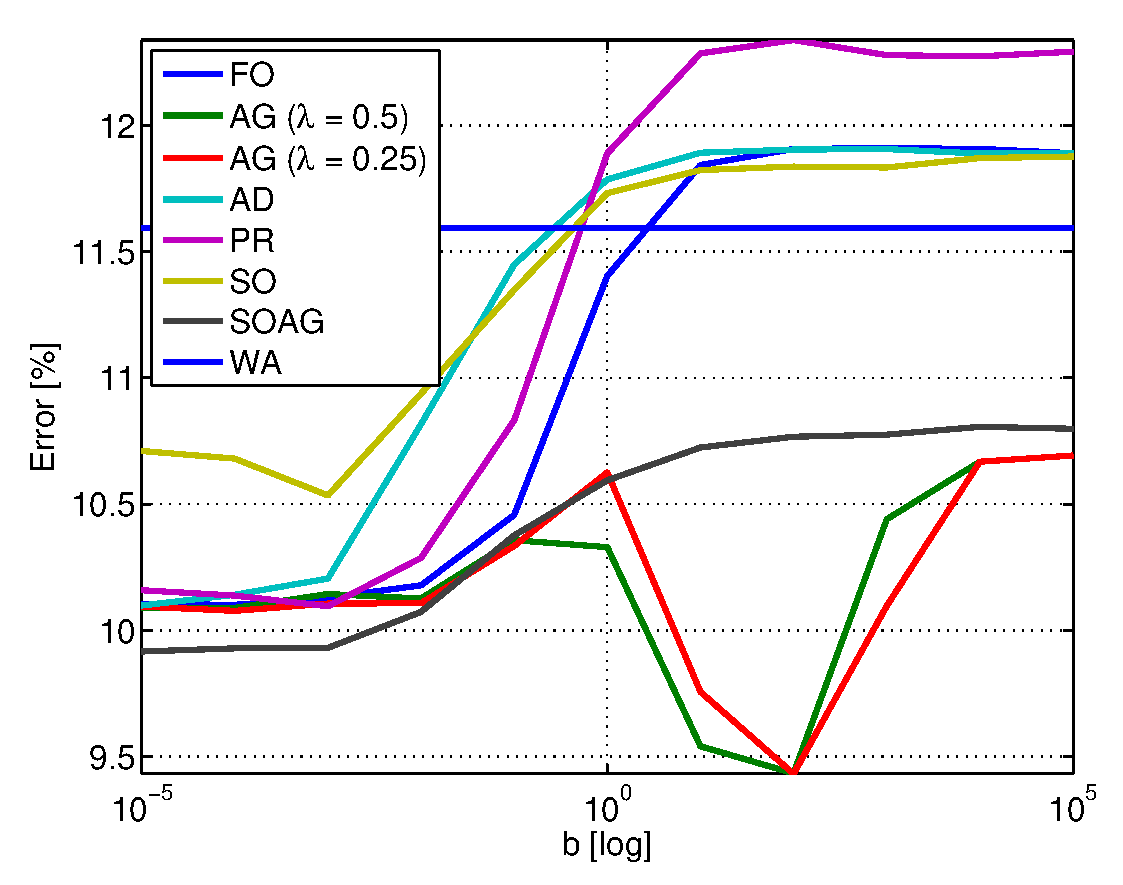
\includegraphics[width=0.5\textwidth]{figs/test-v1.eps}

\end{centering}

\end{frame}




\begin{frame}{VJ Multiclass - Test errors}
$1-vs-1 weak$ gives the best results on VJ settings since it updates also when 
there is no  correct prediction.

\begin{centering}
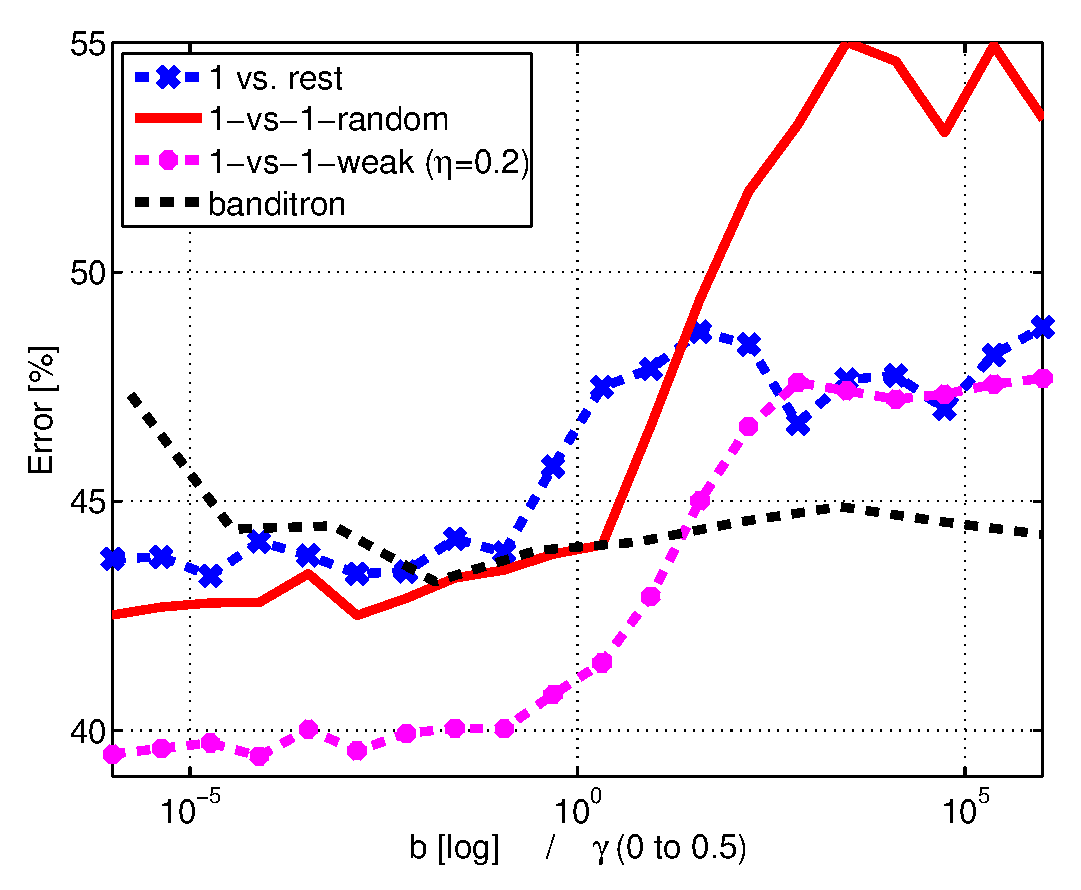
\includegraphics[width=0.6\textwidth]{figs/VJ_three_methods.eps}

\end{centering}
\end{frame}


% \begin{frame}{Test and train error vs. b}
% \textbf{NLP Data - 2 hard tasks, 3 easy, second order } \newline
% The train error is what we bound\newline
%
% \begin{centering}
% 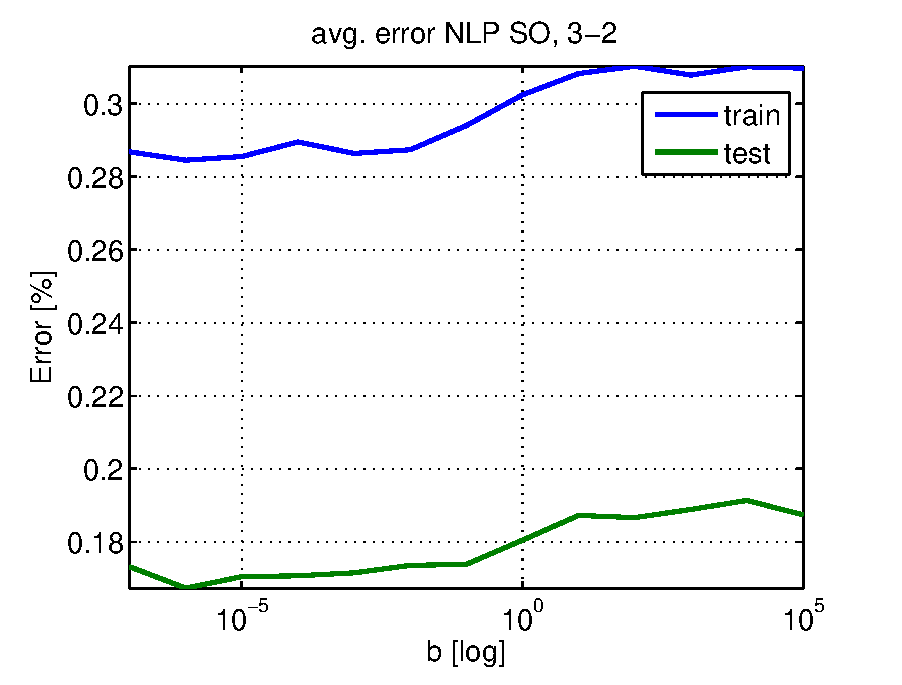
\includegraphics[width=0.6\textwidth]{figs/NLP_SO_3_2_mean_error.eps}
%
% \end{centering}
% \end{frame}

%\begin{frame}{Adaptive $b$}
%\textbf{USPS, One vs. One data} \newline
%The plots show mean error for adaptive $b$ algorithm with $b_{i,t}= (N_{i,t})^{\kappa}(\sum_t{Z_{i,t}})^{\eta}$\newline
%Where $N_{i,t}$ is the number of updates on task $i$ up to time $t$.\newline
%
%We see that a good choice is  $b_{i,t}=\sqrt{(N_{i,t})/(\sum_t{Z_{i,t}})}$\newline
%
%\begin{centering}
%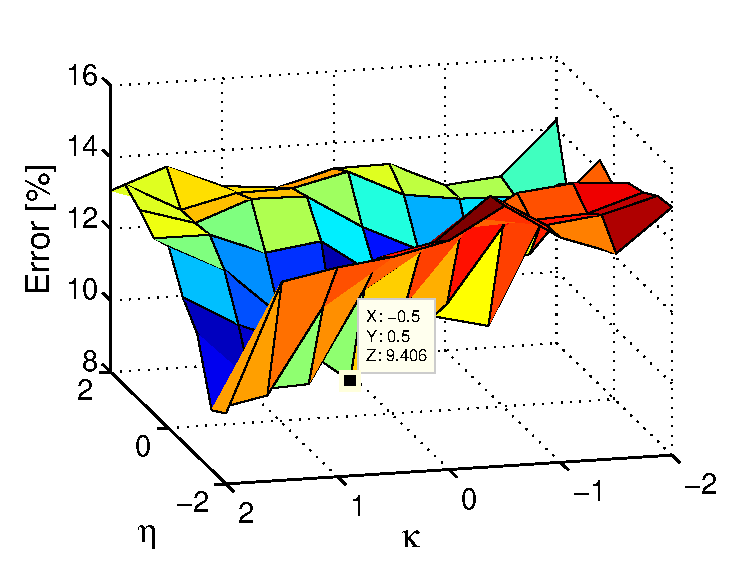
\includegraphics[width=0.5\textwidth]{figs/Mean_test_error_adaptive_b_V2_3D.eps}
%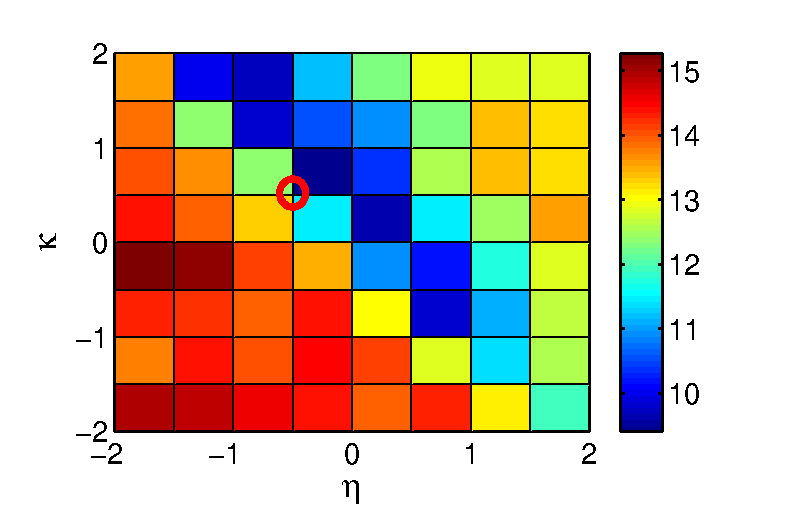
\includegraphics[width=0.5\textwidth]{figs/Mean_test_error_adaptive_b_V2_2D.eps}
%\end{centering}
%\end{frame}
%
%\section{Conclusion}

\begin{frame}{Conclusion}
\begin{itemize}
\item We introduced algorithms to solve the multi-task learning with a shared annotator\newline
\item We analyzed the algorithms in the mistake bound model  \newline
\item We showed a variation of our SHAMPO algorithms to contextual bandits - decoupling of exploration and exploitation.\newline
\item Experiments that show that SHAMPO algorithms can acheive good results even with partial feedback and focuses on the hard tasks, were presented. \newline
\end{itemize}
\end{frame}

\begin{frame}{Thanks }
\begin{itemize}
\item Prof. Koby Crammer for  the guidance and  supervising\newline
\item My beloved wife Zohar, for the support\newline
\item My friend  from the machine learning group\newline
%\item Intel  for the generous sponsoring
\end{itemize}

\end{frame}

\begin{frame}{~}
\begin{center}
\begin{Huge}Questions ???\end{Huge}
\end{center}
\end{frame}

\end{document}
